%%%%%%%%%%%%%%%%%%%%%%%%%%%%%%%%%%%%%%%%%%%
%
% szablon pracy licencjackiej 
% korzystający ze stylu pracalicmgr.cls
% 2017.03.01 P. Durka durka@fuw.edu.pl 
% na podstawie pliku J. Żygierewicz 2016
%
%%%%%%%%%%%%%%%%%%%%%%%%%%%%%%%%%%%%%%%%%%%



\documentclass{pracalicmgr}
\usepackage{polski}
\usepackage[utf8]{inputenc}

\usepackage{graphicx}
\usepackage{multicol}
\usepackage{caption}
\usepackage{subcaption}


\usepackage{float}
\graphicspath{ {./images/} }

%\usepackage[round]{natbib}   % omit 'round' option if you prefer square brackets
%\bibliographystyle{plainnat}
\usepackage[maxcitenames=2, backend=biber, style=authoryear]{biblatex}
\renewcommand*{\nameyeardelim}{\addcomma\space}
%\renewcommand*{\nameyeardelim}{\addcomma\space}

\usepackage{ gensymb }

\renewcommand{\contentsname}{Table of contents}
\renewcommand{\listtablename}{List of tables}
\renewcommand{\listfigurename}{List of figures}
\renewcommand{\chaptername}{Chapter}
\renewcommand{\tablename}{Table}
\renewcommand{\figurename}{Figure}
\renewcommand{\appendixname}{Appendix}
\renewcommand{\abstractname}{Summary}



\author{Agnieszka Wierzbicka}

\nralbumu{323371}


\title{Analysis of laminar profile of evoked potentials in rat visual cortex}

\tytulang{Analiza profilu warstowego potencjałów wywołanych w korze wzrokowej szczura}

\kierunek{Applications of Physics in Biology and Medicine}

\specjalnosc{Neuroinformatics}

\opiekun{Jarosław Żygierewicz, Ph.D. 
	\\Biomedical Physics Division
	\\Instytute of Experimental Physics
	\\Faculty of Physics, University of Warsaw
	\\and
	\\prof. Wioletta Waleszczyk
	\\Laboratory of Visual Neurobiology
	\\Department of Neurophysiology
	\\Nencki Institute of Experimental Biology PAS }

%\dziedzina{13.200}
\dziedzina{13.2 Physics}

\date{December 2017}

\keywords{po polsku czy po ang?}

\bibliography{bibliografia}

\begin{document}


    \maketitle
    \let\cleardoublepage\clearpage
    
    \begin{abstract}
Krótkie (maks. 800 znaków) streszczenie pracy, na przykład:

Lorem ipsum – tekst składający się z łacińskich i quasi-łacińskich wyrazów, mający korzenie w klasycznej łacinie, wzorowany na fragmencie traktatu Cycerona „O granicach dobra i zła” (De finibus bonorum et malorum) napisanego w 45 r. p.n.e. Tekst jest stosowany do demonstracji krojów pisma (czcionek, fontów), kompozycji kolumny itp. Po raz pierwszy został użyty przez nieznanego drukarza w XVI w.

Tekst w obcym języku pozwala skoncentrować uwagę na wizualnych aspektach tekstu, a nie jego znaczeniu.


     \end{abstract}

  
    \tableofcontents
    
    \chapter*{Goal}
    \addcontentsline{toc}{chapter}{Goal}
    The main goal of this work was to study responses of neurons from particular layers of visual cortex to visual stimulation with different temporal frequency.
    
    \chapter{Introduction}
    
    \section{Structure of the visual system}
    Visual perception is an ability to process information coded by light. There are two largely independent visual pathways. Both begin in retina where light is converted into electrical discharge by photoreceptors and then thew information is transferred to ganglion cells and then further via the optic nerve (Fig.~\ref{rys:neural_circuitry}). Here the pathways split. The first one, known as geniculate visual pathway, leads via the dorsal part of lateral geniculate nucleus (LGN) to primary visual cortex (VCx), and from there further to higher-order cortex. The second pathway, known as extrageniculate visual pathway, leads through superior colliculus and the lateral posterior nucleus-pulvinar complex and then---similarly to the first pathway---reaches primary visual cortex and the higher-order cortex.(\cite{viola}, \cite{thomsonlayer6}). 
    \begin{figure}[htbp]
    	\begin{center}
    		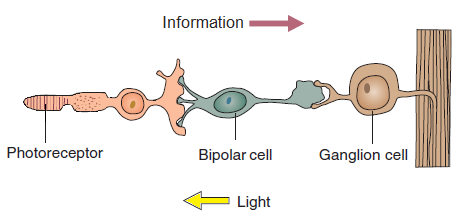
\includegraphics[scale=0.9]{neural_circuitry.png}
    	\end{center}
    	\caption{Neural circuitry in the retina (modified from \cite{carlsonphysiology}).}
    	\label{rys:neural_circuitry}
    \end{figure}      

   \section{Parallel processing in the visual system}
    Retina is the first place where visual information is decoded and segregated. Three main morphological types of ganglion cells recognize different properties of visual stimuli (Fig. \ref{rys:ganglio}).

	\begin{figure}[H]
	\begin{subfigure}{.33\textwidth}
		\centering
		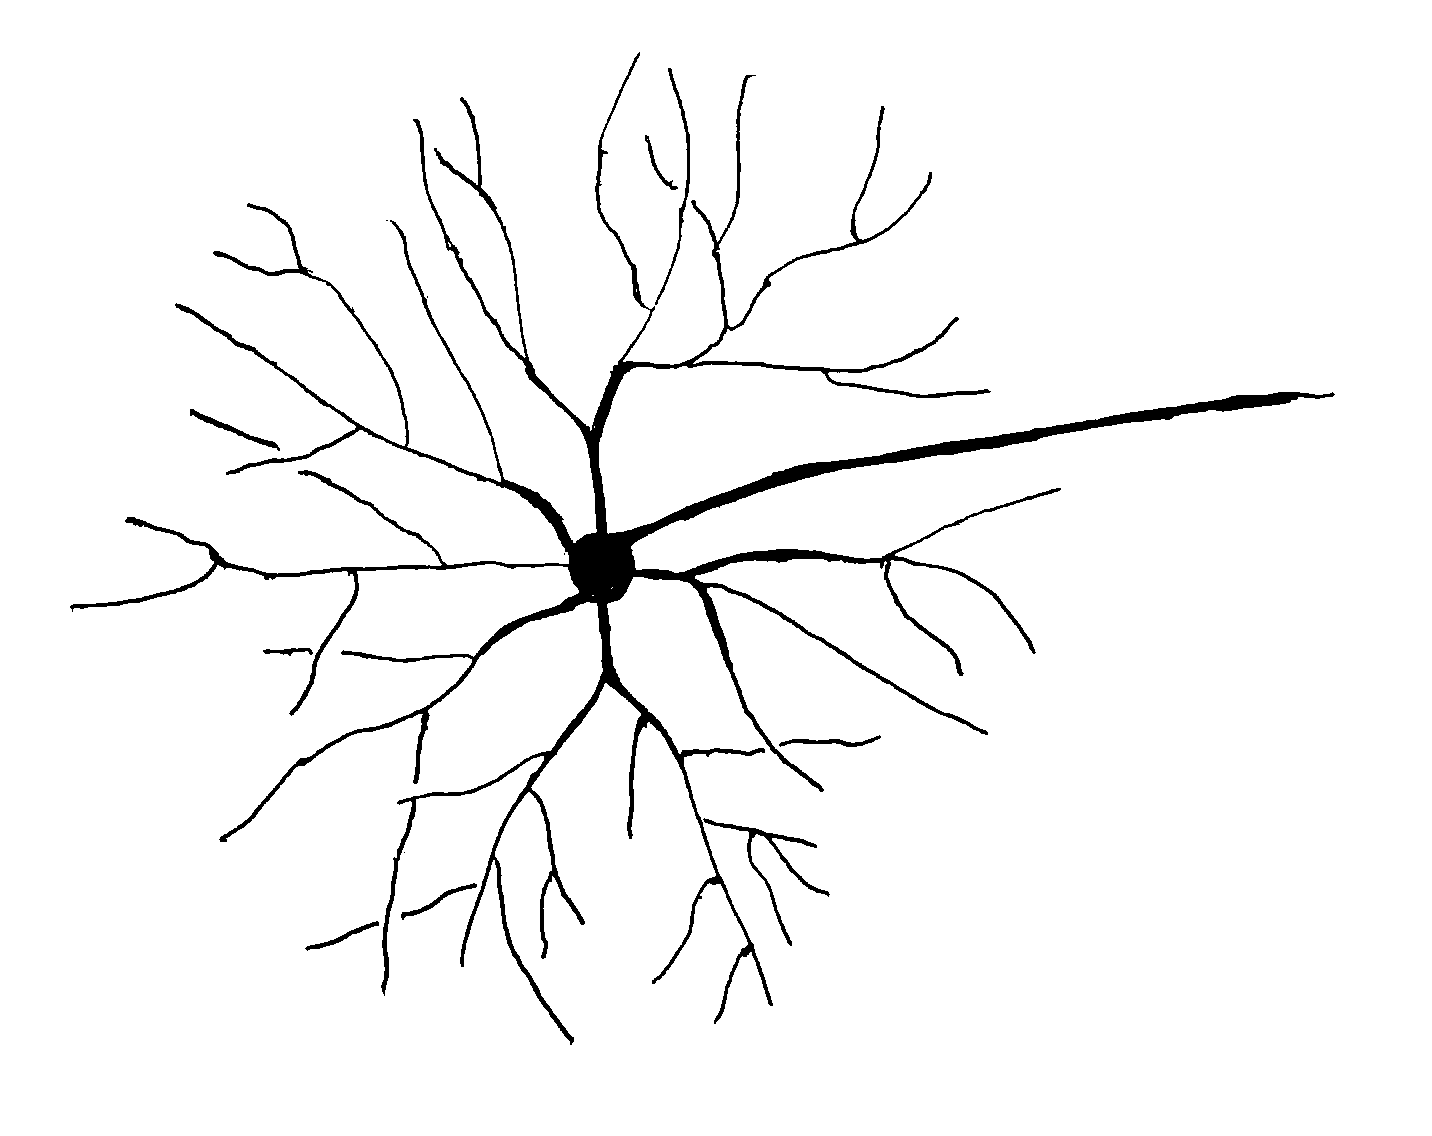
\includegraphics[width=1.\linewidth]{cell_M2.png}
		\caption{Magnocellular}
		\label{rys:magno}
	\end{subfigure}%
	\begin{subfigure}{.33\textwidth}
		\centering
		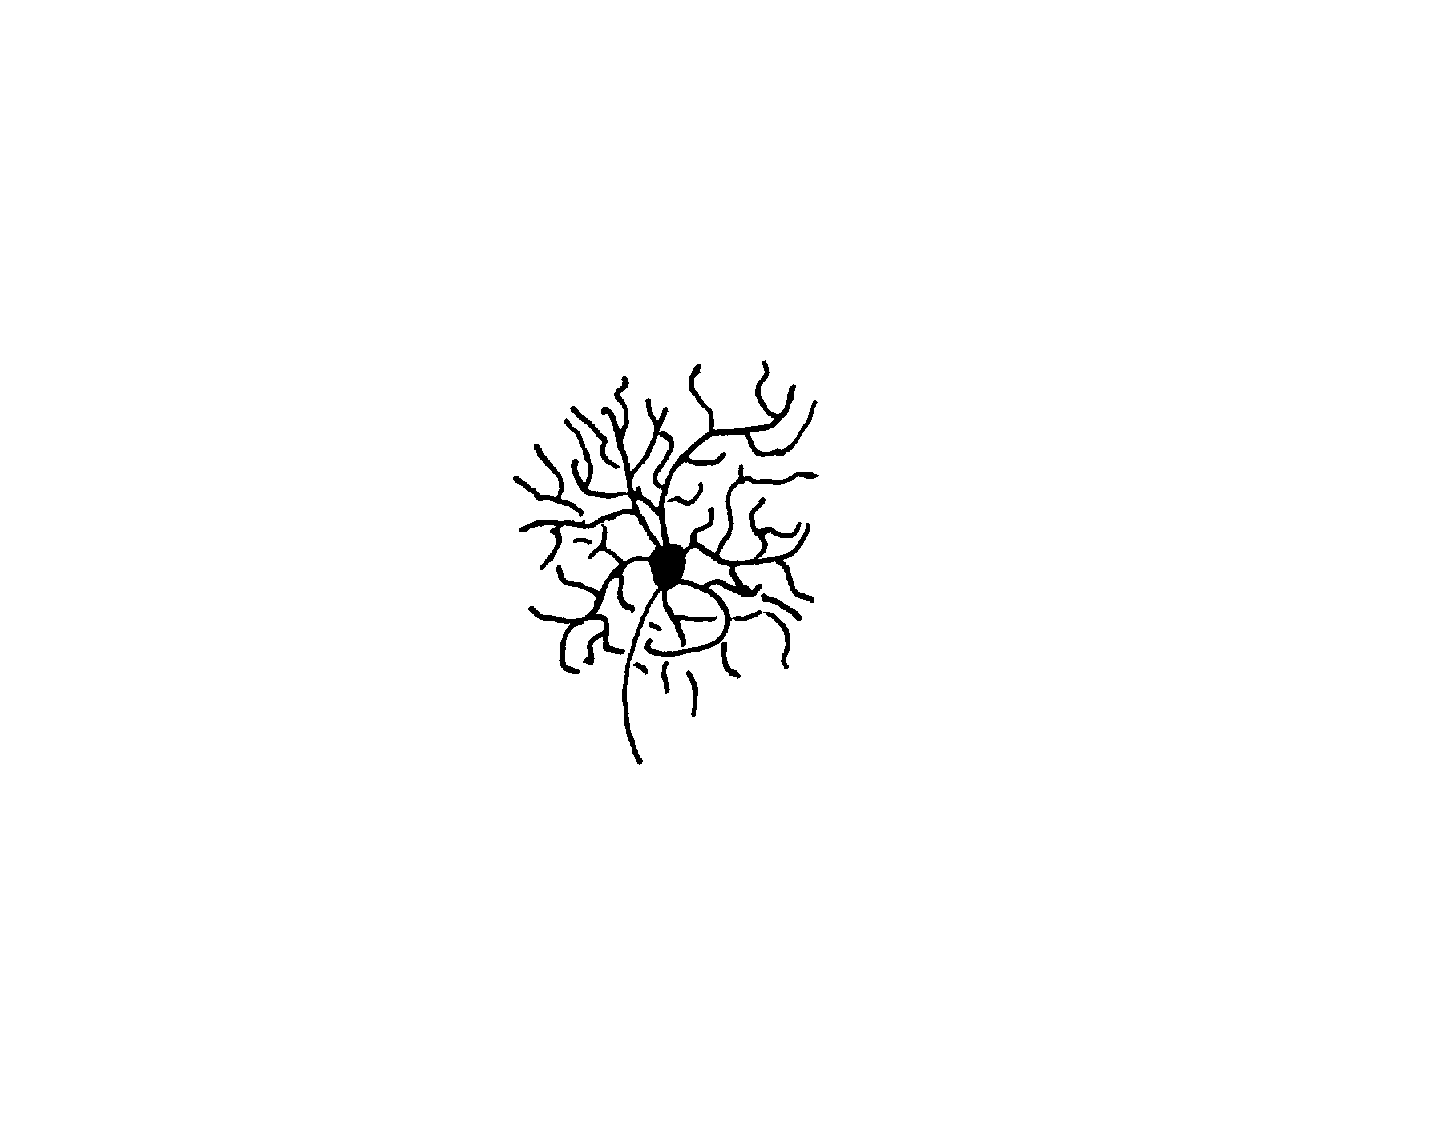
\includegraphics[width=1\linewidth]{cell_P2.png}
		\caption{Parvocellular}
		\label{rys:parvo}
	\end{subfigure}
	\begin{subfigure}{.33\textwidth}
	\centering
	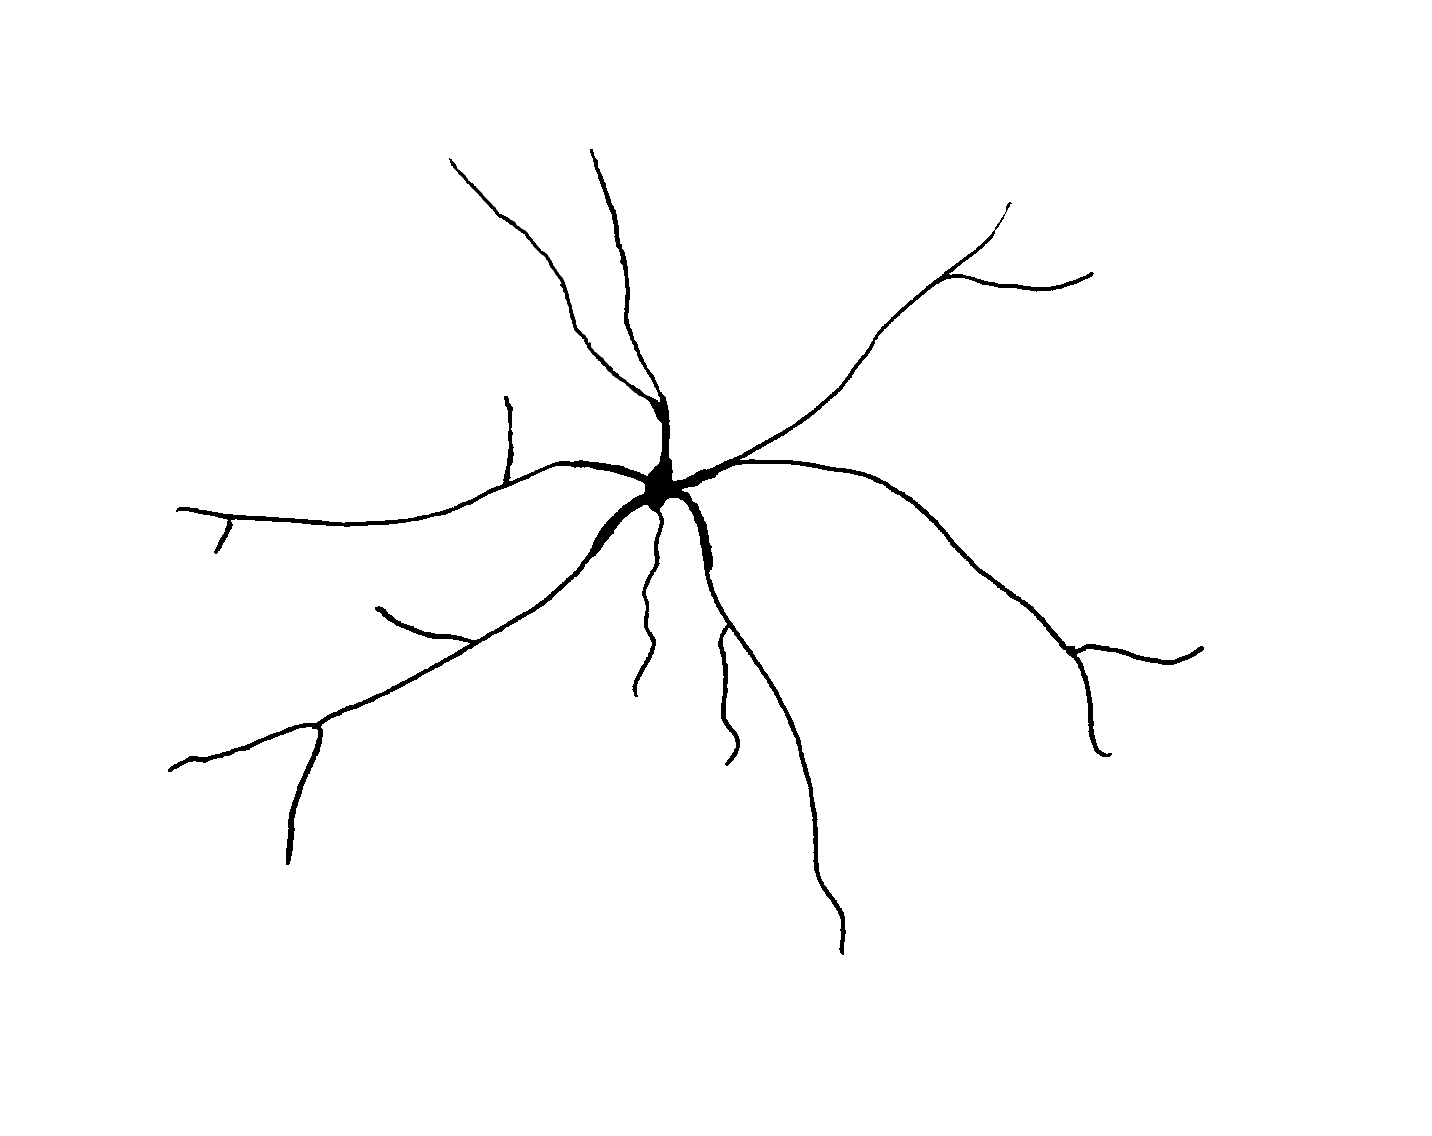
\includegraphics[width=1\linewidth]{cell_K2.png}
	\caption{Koniocellular}
	\label{rys:konio}
	\end{subfigure}
	\caption{Three most important morphological classes of ganglion cells  (Drawing on the basis of \cite{parallel}).}
	\label{rys:ganglio}
	\end{figure}
	 Magnocellular cells (Fig. \ref{rys:magno}) have big soma with large dendritic tree. Thanks to lthick axon this type of cells can recognize fast stimuli but have poor spatial frequency. Parvocellular cells are cells with medium soma (Fig. \ref{rys:parvo}). They are characterized by high resolution spatial frequency due to small dendritic size, but weak temporal frequency resolution. Koniocellular cells are heterogeneous group of cells with small-to-medium somata of different dendritic morphologies (Fig. \ref{rys:konio}; \cite{parallel}, \cite{viola}). 
	
	
    \section{Architecture of primary visual cortex}
     Primary visual cortex can be divided into 6 vertical layers differing from one another in function and morphology. Sometimes layers II and III are considered to be one layer II/III (Fig. \ref{rys:lgn}).
	(\cite{viola})
    \begin{figure}[H]
	\begin{center}
		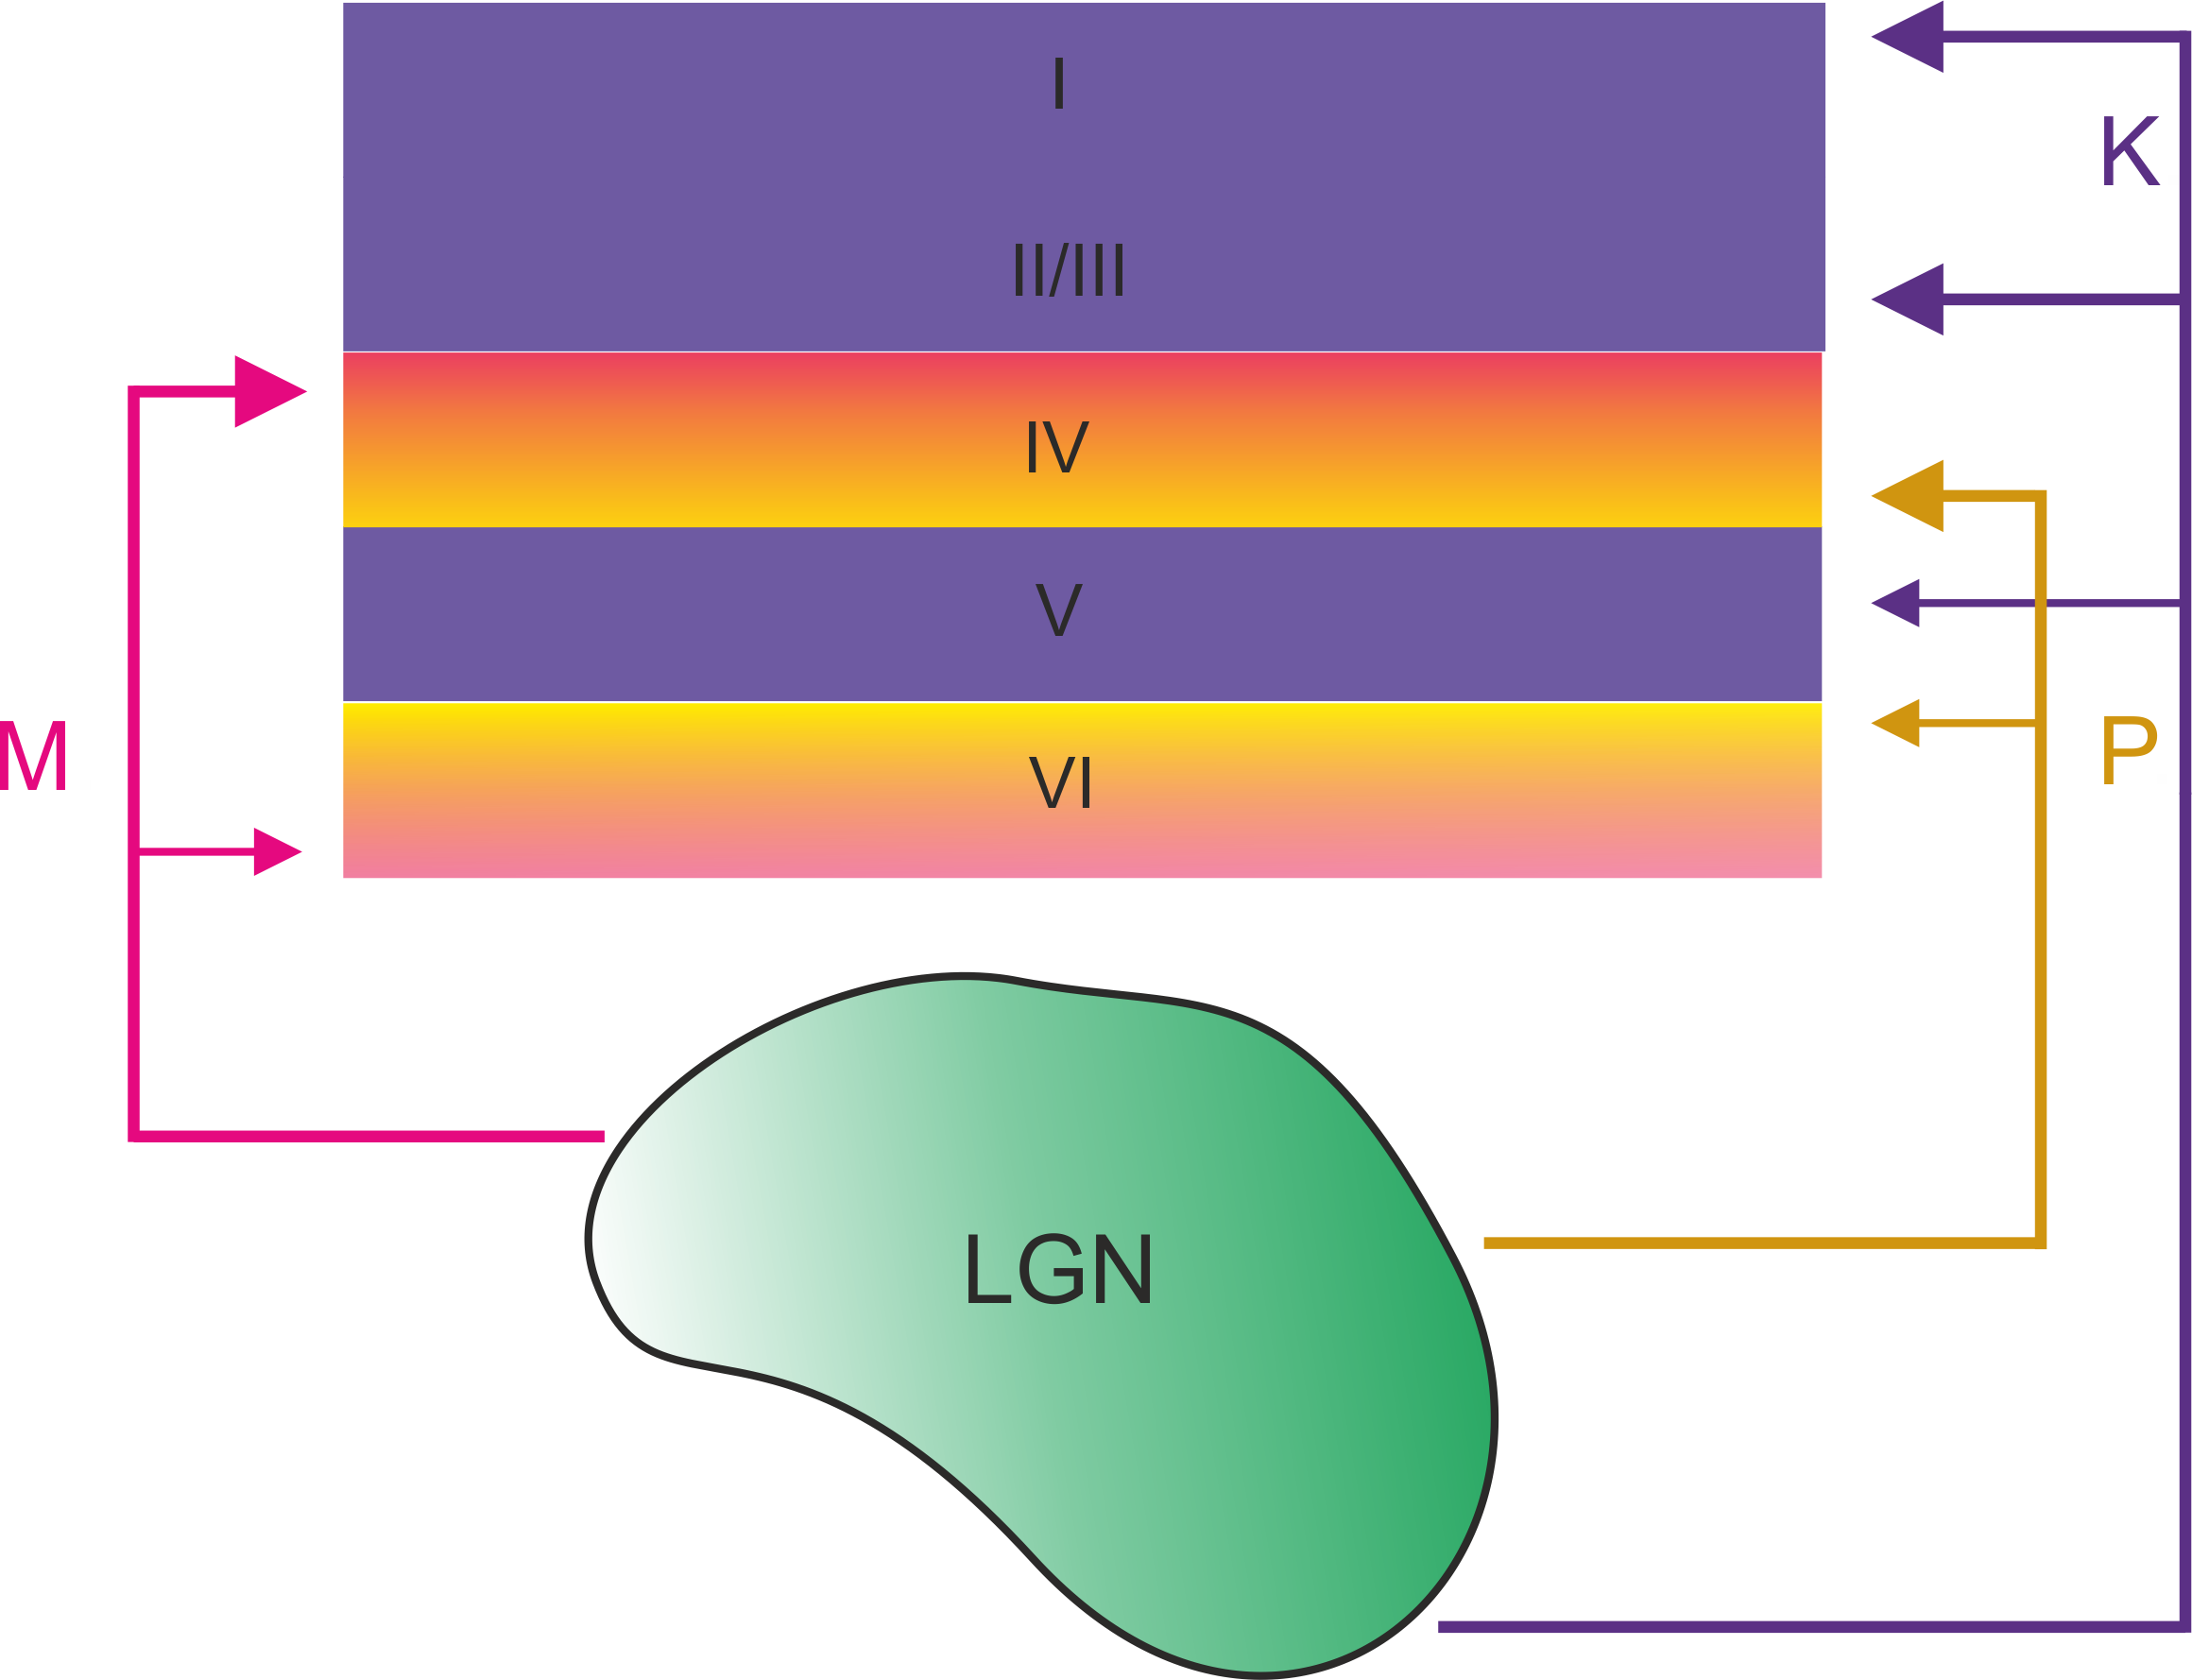
\includegraphics[scale=0.4]{aga_LGN.png}
	\end{center}
	\caption{The main connections made by axons from the dorsal lateral geniculate body to primary visual cortex.}
	\label{rys:lgn}
	\end{figure}  

        First main division is made based on granule cells located in layer IV. These cells are characterized by very small cell bodies. Layers above IV are called \emph{supragranular} while layers below are referred to as \emph{infragranular}. As it was shown (by \cite{maier2010}), around layer IV there is a polarization change observable on averaged evoked potentials chart. In layer I cell bodies are absent but there are plenty of axons, dendrites, and synapses. Two major classes of cortical cells are pyramidal cells which occur in all layers except I and IV, and stellate cells which are found in all layers (Fig. \ref{rys:morphology_neurons}).
        
        \begin{figure}[H]
        	\begin{center}
        		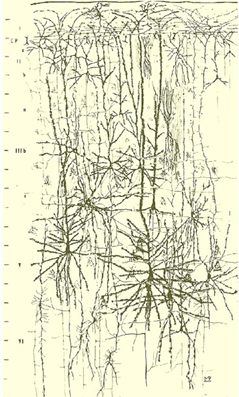
\includegraphics[scale=1]{morphology_neurons.png}
        	\end{center}
        	\caption{Composite figure of a mosaic of camera lucida drawings showing the morphological features (size, location, and distribution) of the principal neuronal types of the human cortex. From rapid-Golgi preparations. Scale (on the left): 100 $\mu$m  (\cite{morphology}).}
        	\label{rys:morphology_neurons}
        \end{figure}   
             
        
        \section{Local field potentials (LFPs)}
        Electrophysiology is a method to record activity of the brain with high temporal resolution and weaker spatial. Thanks to electrodes spread in different places on the brain we can gather information from them. It can be used to check the response for various stimuli at different locations. Usage of vertical electrodes allows to record simultaneously signal across the brain. Nearly all visual information enters the cortex via area VCx. 
        
        Local field potentials (LFP), the low-frequency part of extracellular electrical
        recordings, are a measure of the neural activity reflecting dendritic
        processing of synaptic inputs to neuronal populations. LFP consisted of postsynaptic and action potentials  (Fig. \ref{rys:VCx_LFPs}).
        
        // Electrocorticogram is the signal gathered from the cortex and the subcortical structures. Electrodes placed next to neurons allow recording brain activity from a small region which is called local field potential (LFP). //
        \begin{figure}[htbp]
        	\begin{center}
        		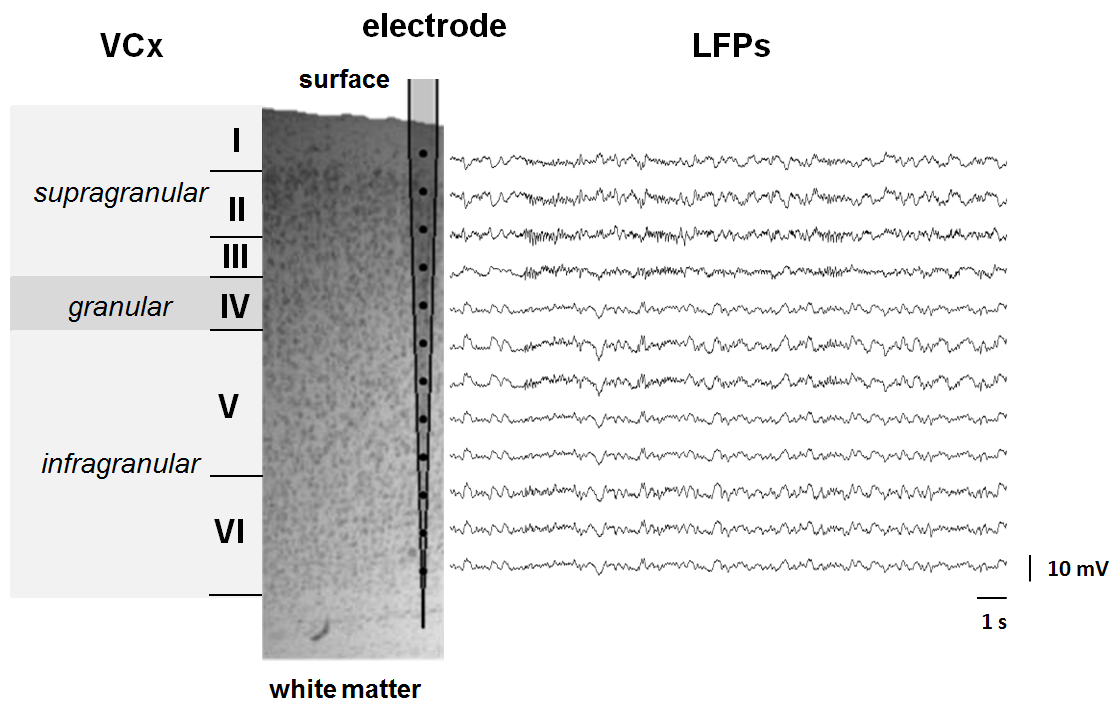
\includegraphics[scale=0.5]{VCx_LFPs2.png}
        	\end{center}
        	\caption{ An example of LFP signal in VCx.}
        	\label{rys:VCx_LFPs}
        \end{figure} 
        
        Postsynaptic potentials are potentials reaching dendrite of nerve cell. They can be either excitatory (Excitatory Post-Synaptic Potentials, EPSPs) that enhance chance of induces action potentials or inhibitory (Inhibitory Post-Synaptic Potentials, IPSPs) which that making action potential less likely to happen. Lots of potentials reach neuron. When summary of them reach threshold neuron becomes excited and generate action potential which propagates along axon (Fig. \ref{rys:PSPs}).
        \begin{figure}[htbp]
        	\begin{center}
        		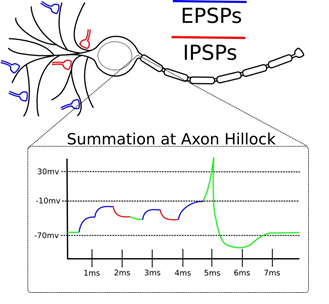
\includegraphics[scale=1]{PSPs.png}
        	\end{center}
        	\caption{Excitatory and inhibitory post-synaptic potentials.}
        	\label{rys:PSPs}
        \end{figure} 
        
\chapter{Materials and methods}   
 	\section{Subjects}
 	All experimental procedures  were performed conducted in accordance with the ARVO Statement for the Use of Animals in Ophthalmic and Vision Research and  the EC Directive 86/609/EEC for animal experiments using protocols and methods accepted by the First Warsaw Local Ethical Commission for Animal Experimentation. The experiments took place in Neurobiology of Vision Laboratory in Nencki Institute with great help from mgr Katarzyna Kordecka.
 	For electrophysiological experiments presented in this study, we used 6 adult male Wistar rats (250-300g). All animals were housed with free access to food and water and maintained on a 12 h light/dark cycle.
 	
 	\section{Surgical procedures}
 	Animals were under deep urethane anesthesia (1.5 g/kg, Sigma-Aldrich, Germany, 30\% aqueous solution, i.p) and placed in a stereotaxic apparatus. Additional doses of urethane (0.15 g/kg) were administered if it was such a necessity. Body temperature was maintained between 36 and 38 \degree C using an automatically controlled electric heating blanket. Every hour fluid requirements were fulfilled by subcutaneous injections of 0.9\% NaCl (1ml/hour) and eyes were humidified with Vidisic (Polfa Warszawa S.A., Poland) to prevent cornea from drying. The skin on the head was disinfected with iodine and local anesthetic of 1\% lidocaine hydrochloride (0.5 ml, Polfa Warszawa S.A., Poland) was injected over the scalp. The skull was opened to expose areas of the binocular primary VCx (7.5 mm posterior to bregma, 5.0 mm lateral) in left hemisphere. Coordinates were chosen based on the rat brain atlas of Paxinos and Watson (\cite{atlas}). 
 	
 	\section{Electrophysiology recording}
 	In the experiments stimuli were presented with interstimulus intervals (ISI) of  1, 0.5, 0.25, 0.2, 0.143, 0.08 [s] which corresponds to frequencies 1, 2, 4, 7, 10, 12 [Hz], respectively. An individual stimulus was a 2-millisecond-long LED flash at 560 cd/m2 luminance. There was dark in the room and rats had both eyes opened. For each frequency the stimuli were applied in 40 repetitions of 5-second-long chunks with random (2-3 s) breaks between them (Fig. \ref{rys:stimuli}).
 	\begin{figure}[htbp]
 		\begin{center}
 			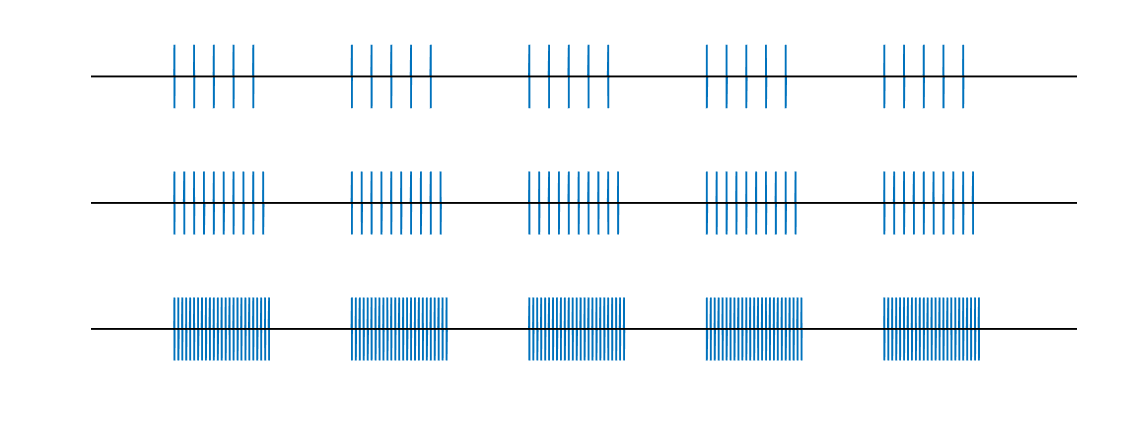
\includegraphics[scale=0.5]{stimuli.png}
 		\end{center}
 		\caption{ The stimuli were presented in 5 s long series at given frequency (from 1 to 12 Hz). The number of chunks was always 40 and number of stimuli depended on frequency.}
 		\label{rys:stimuli}
 	\end{figure} 

    \chapter{Data analysis}
    \section{Description averaging visual potentials}
    Visual Evoked Potential (VEP) is a case of steady state evoked potential where light is a stimulus. In theory spontaneous activity of ECoG is a stochastic process (independent, stationary noise with mean equal to zero) and brain response to each stimulus is constant. In that way signal in each realization can be expressed by  
    \begin{equation}
    x_i(t) = s(t) + n_i(t),
    \end{equation}
    where s(t) is a real signal, ni(t) noise part. For white noise with mean zero, expected value equals:
    \begin{equation}
    E\left[ \frac{1}{N}\sum_{i=1}^{N} n_i(t)\right] = 0, 
    \end{equation}
    which causes that for averaged signal: $E\left[ \bar{x}(t) \right] = s(t).$
    
    \section{Usage of method}
    Data from each record was averaged by trials and 7 channels out of 12 were chosen to obtain representative profile: 3 of supragranular, 3 of infragranular and one channel from granular layer (layer IV,  Fig \ref{rys:wybieranie_kanalow}).
     
    \begin{figure}[H]
    \begin{center}
    		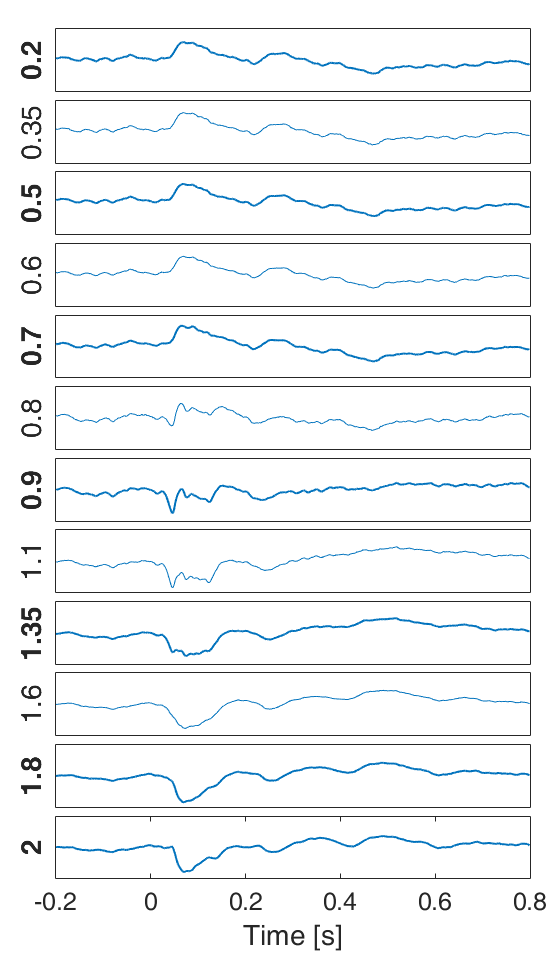
\includegraphics[scale=0.5]{wybieranie_kanalow.png}
    	\end{center}
    	\caption{ Representative averaged evoked potentials from V1. On channels at 0.8 and 0.9 mm depth repolarization can be observed. Channels chosen to further analysis are marked in bold. Time 0 s means an occurrence of stimulus.}
    	\label{rys:wybieranie_kanalow}
    \end{figure} 

	After each repetition of stimuli there are two deflection of mean visible. First deflection starts nearly immediately after stimulus - second after around 0.3 s  Further they are called first and second peaks (no matter whether they are negative or positive, Fig. \ref{rys:piki}). For stimulation of 2 Hz there is also visible another peak for the next stimulus at 0.5 s (Fig \ref{rys:piki_2Hz}). 
	
	\begin{figure}[H]
		
	\begin{subfigure}{.5\textwidth}
	\centering
	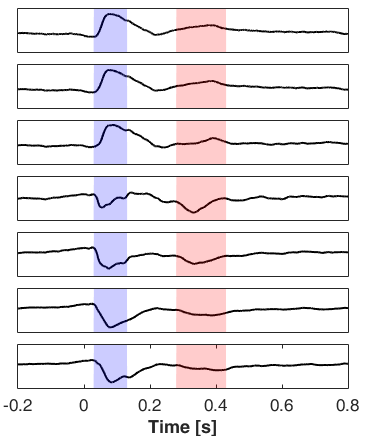
\includegraphics[width=0.8\linewidth]{wybieranie_1Hz.png}
	\caption{Stimulation of 1 Hz.}
	\label{rys:piki_1Hz}
	\end{subfigure}
	\begin{subfigure}{.5\textwidth}
	\centering
	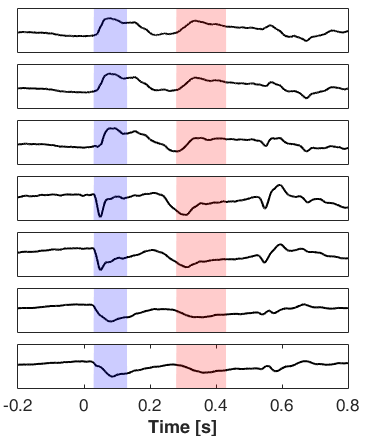
\includegraphics[width=0.8\linewidth]{wybieranie_2Hz.png}
	\caption{Stimulation of 2 Hz.}
	\label{rys:piki_2Hz}
	\end{subfigure}
	\caption{Averaged signal after 40 repetitions of stimuli.}
	\label{rys:piki}
	\end{figure}

    \section{Welch}
    The method, introduced by Welch (\cite{welch}),  relies  on splitting the signal into overlapping time windows, estimation of the periodogram for each of the windows, and then averaging of the estimates. Estimation of power spectrum density was calculated both on averaged by trials data. Hamming window with 3-second duration by 2 seconds was used. 
    
    \section{CSD}
    To localize synaptic dynamics, it is convenient, whenever possible, to estimate the density of transmembrane current sources (CSD) generating the LFP.
    
    \chapter{Results}
    Visual response to a single visual stimulus is usually too weak to distinguish from the background of spontaneous activity of visual cortex. Averaging across several repetitions makes evoked potential stand out (Fig. \ref{rys:usrednianie}).
    
        \begin{figure}[H]
    	\begin{center}
    		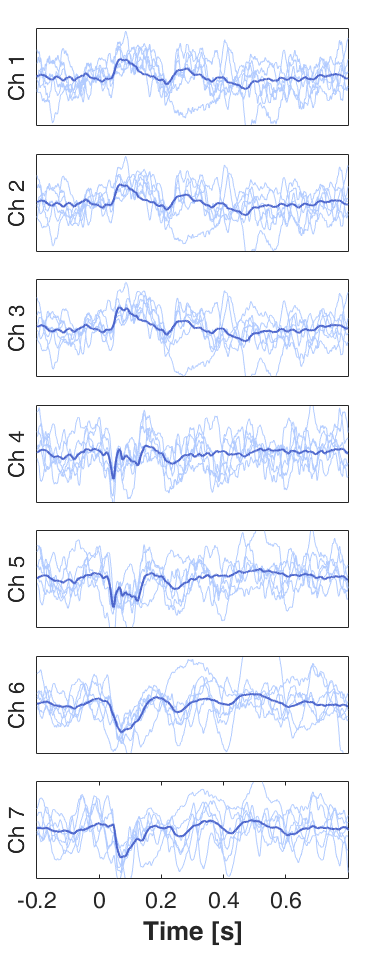
\includegraphics[scale=0.65]{usrednianie3.png}
    	\end{center}
    	\caption{Averaged evoked potentials from VCx for one animal. On channel 4 repolarization can be observed. Y axis is the same for all subfigures. }
    	\label{rys:usrednianie}
    \end{figure} 
    
    \section{Overview of results obtain in the time domain}
    Next, there are all experiments with 6 different stimulation frequency presented one after another. In the Figure \ref{rys:srednie_1_2} results of stimulation with 1 and 2 Hz frequencies are presented---there is a clear peak of response after each repetition of stimulus.
    
    \begin{figure}[H]
    \begin{subfigure}{.5\textwidth}
	\centering
		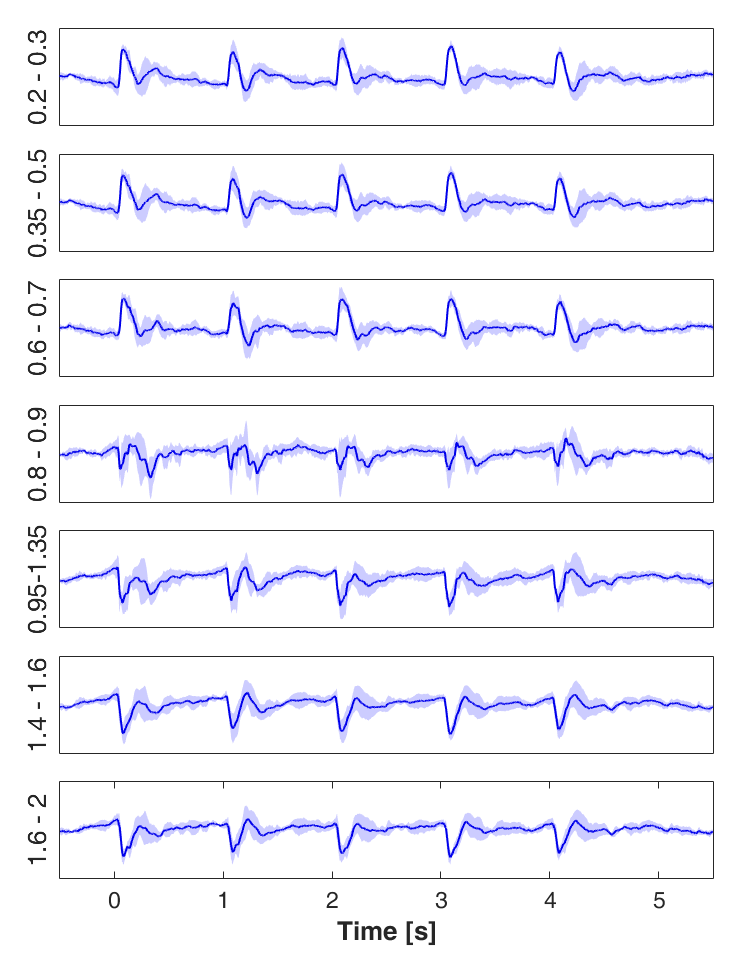
\includegraphics[width=1.\linewidth]{srednie_1Hz_5s.png}
		\caption{Averaged signal for stimulation of 1 Hz.}
		\label{rys:srednie_1Hz}
	\end{subfigure}
	\begin{subfigure}{.5\textwidth}
			\centering
		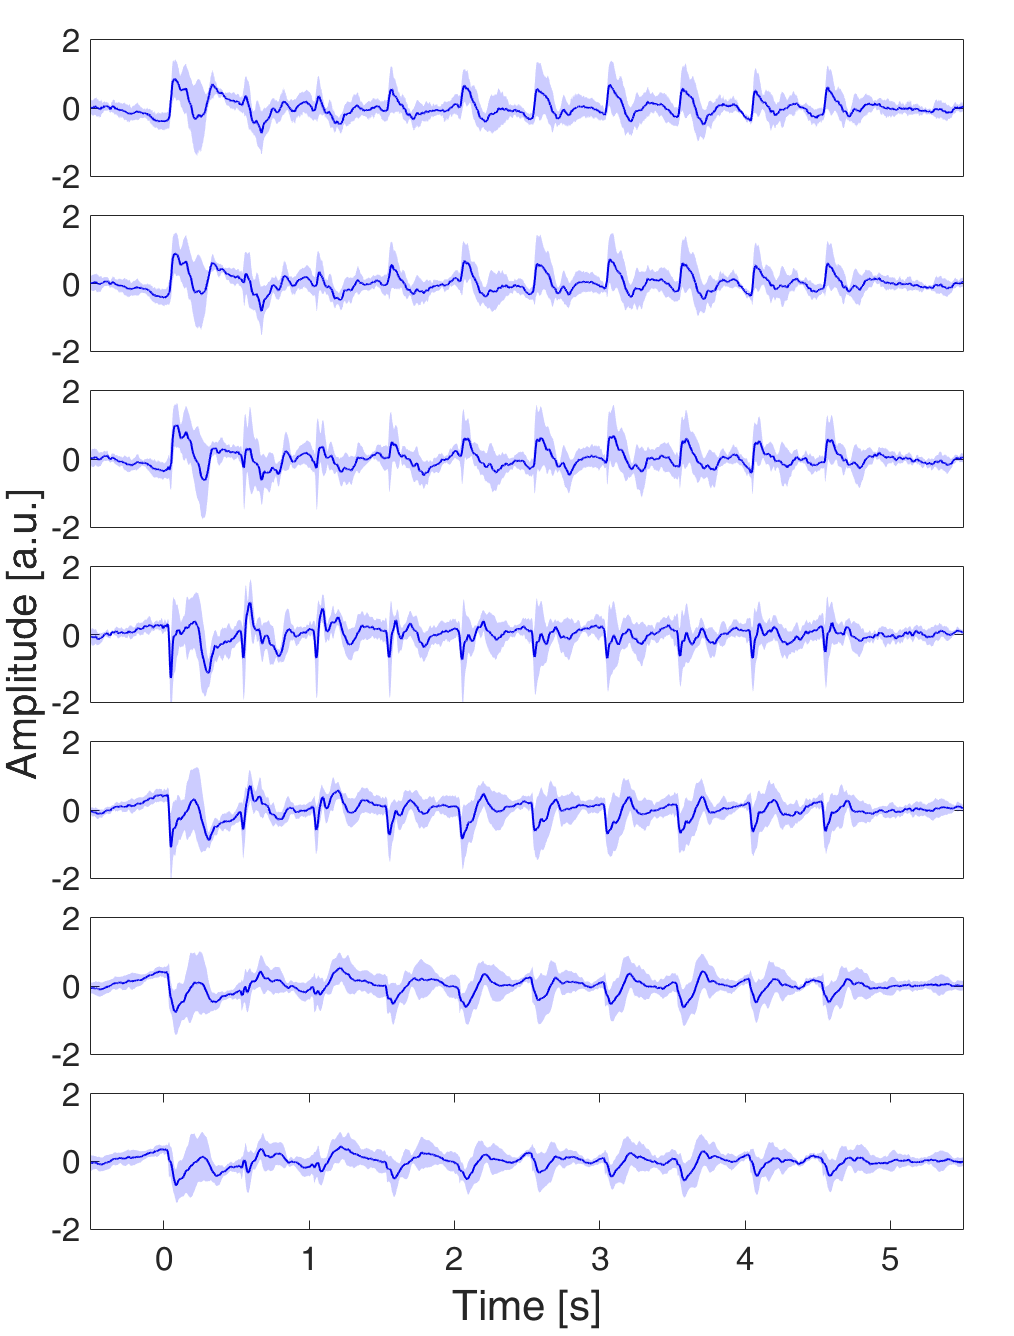
\includegraphics[width=1.\linewidth]{srednie_2Hz_5s.png}
		\caption{Averaged signal for stimulation of 2 Hz.}
		\label{rys:srednie_2Hz}
	\end{subfigure}
	\caption{Averaged signal across 40 repetitions of stimuli.}
	\label{rys:srednie_1_2}
	\end{figure}
    
    For frequencies higher than 2 Hz signals look different (Fig. \ref{rys:srednia_czas}). Firstly the response for stimuli is blurred: stimuli occurs so often that it is impossible to determine where response for certain stimulus starts and ends. The signal forms a continuous oscillation. During the first 1.5 s of the stimulation: the amplitude of oscillations is higher than for the rest. At around 5.1 s there is noticeable peak probably as a response to end of stimulation. 
    
	\begin{figure}[H]
	\begin{subfigure}{.5\textwidth}
		\centering
		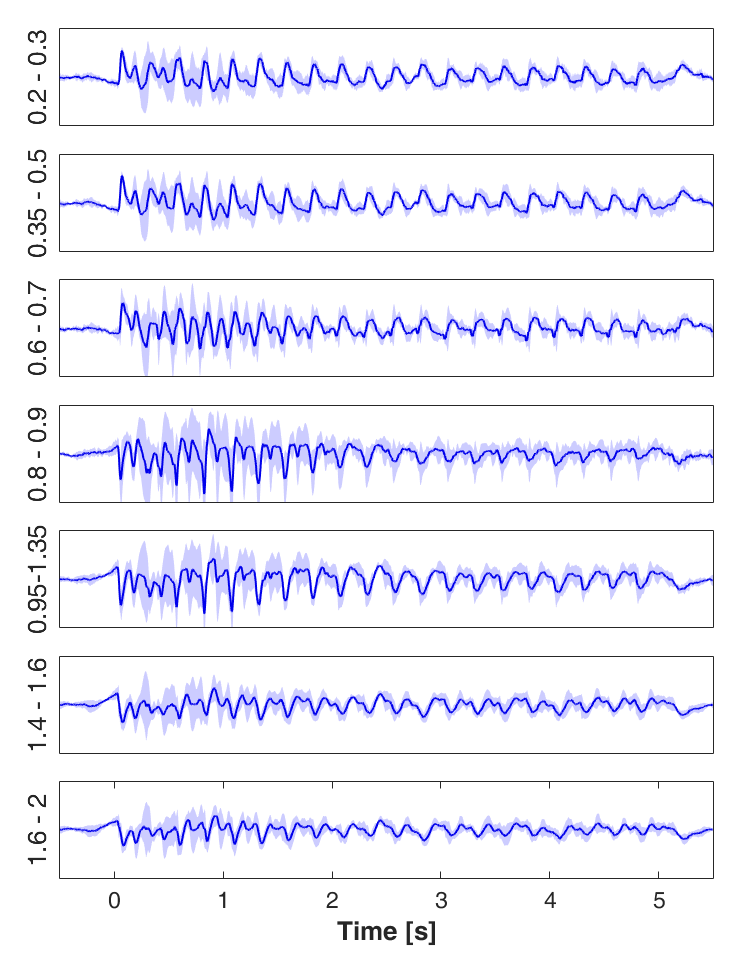
\includegraphics[width=1.\linewidth]{srednie_4Hz_5s.png}
		\caption{Averaged signal for stimulation of 4 Hz.}
		\label{rys:srednie_4Hz}
	\end{subfigure}
	\begin{subfigure}{.5\textwidth}
	\centering
	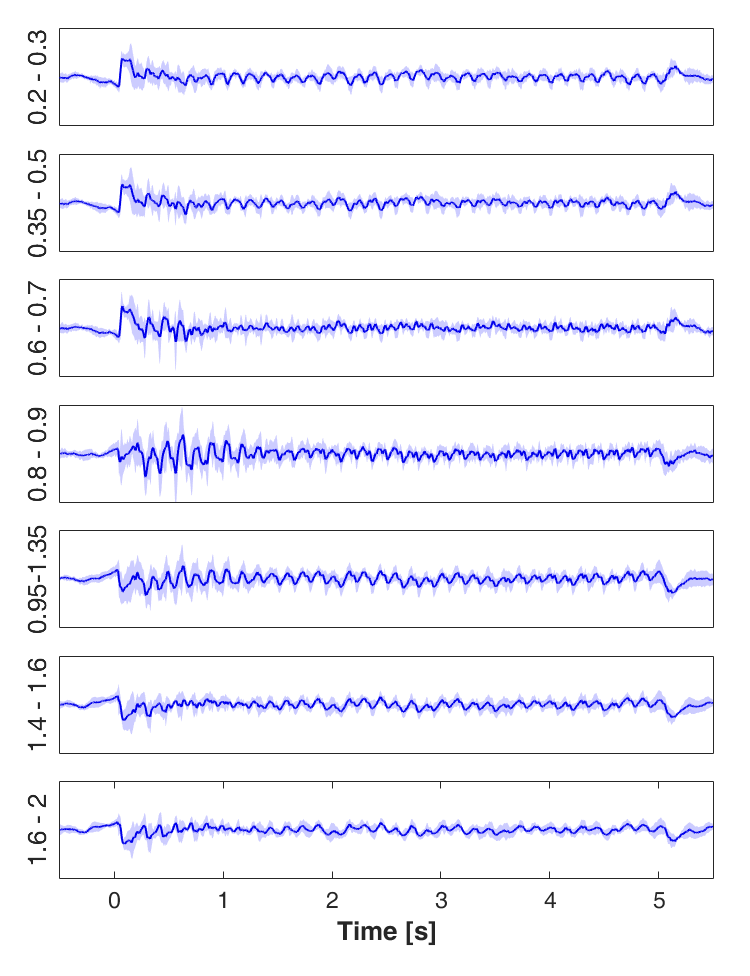
\includegraphics[width=1.\linewidth]{srednie_7Hz_5s.png}
	\caption{Averaged signal for stimulation of 7 Hz.}
	\label{rys:srednie_7Hz}
    \end{subfigure}
	
	\begin{subfigure}{.5\textwidth}
	\centering
	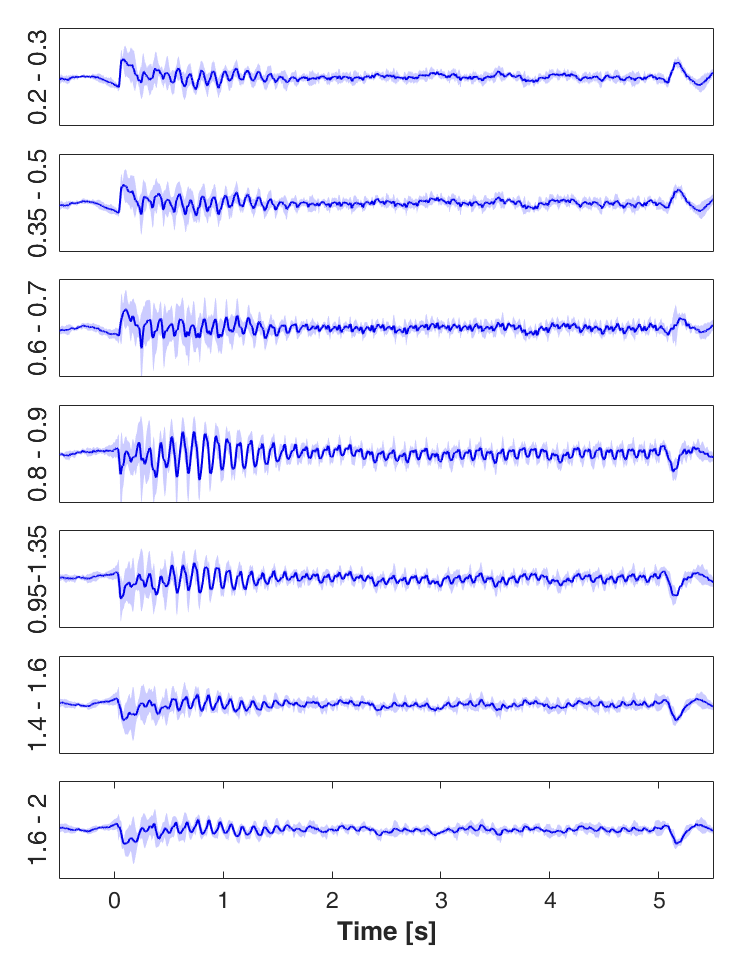
\includegraphics[width=1.\linewidth]{srednie_10Hz_5s.png}
	\caption{Averaged signal for stimulation of 10 Hz.}
	\label{rys:srednie_10Hz}
	\end{subfigure}
	\begin{subfigure}{.5\textwidth}
	\centering
	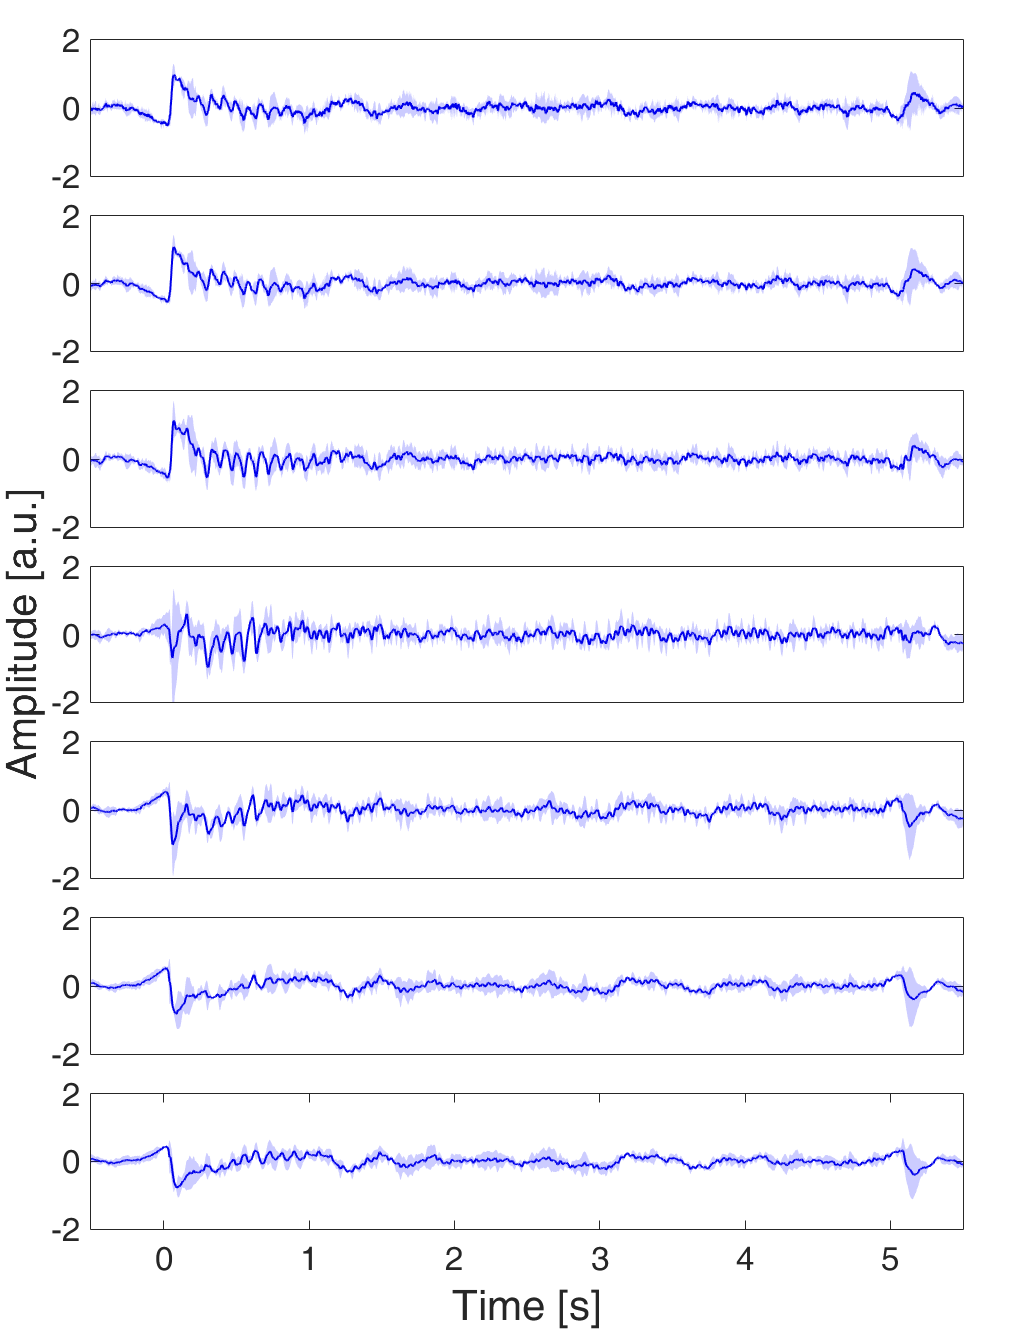
\includegraphics[width=1.\linewidth]{srednie_12Hz_5s.png}
	\caption{Averaged signal for stimulation of 12 Hz.}
	\label{rys:srednie_12Hz}
	\end{subfigure}
	\caption{All experiments averaged by 40 trials in time domain. Point 0 s shows beginning of 5 s constant stimulation. Blue intervals represent standard deviations by the animals. Y axis is the same for all subfigures.}
	\label{rys:srednia_czas}
		
	\end{figure}
	
    \section{Overview of results obtain in the frequency domain}
    
    Next, all power spectra calculated by Welch's methods are shown in Fig. \ref{rys:srednie_widmo}. For stimulation of 1 Hz there are up to 5 harmonic, sometimes even bigger than the fundamental frequency (Fig. \ref{rys:widmo_1Hz}). For frequencies 2 -- 10 Hz, the fundamental frequency and the second harmonic are clean and much bigger than others (Fig. \ref{rys:widmo_2Hz} -- \ref{rys:widmo_10Hz}). Response for 12 Hz in power spectrum is noticeably weaker -- peak in the fundamental frequency is at the same level as low frequency noise (Fig. \ref{rys:widmo_12Hz}).
    
	\begin{figure}[H]
	\begin{subfigure}{.5\textwidth}
		\centering
		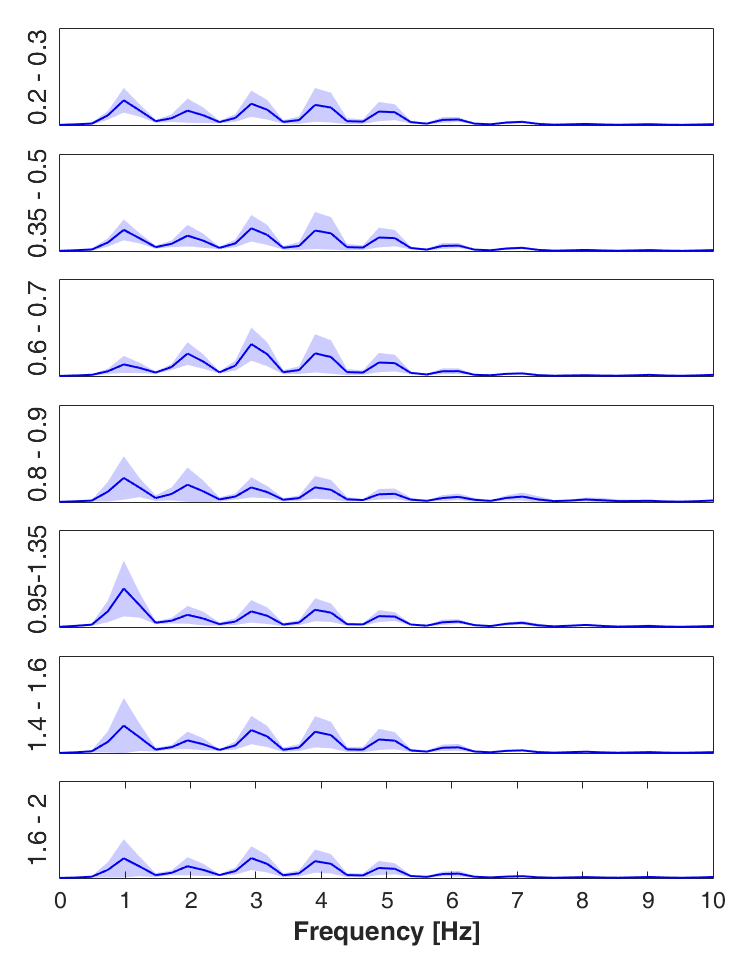
\includegraphics[width=1.\linewidth]{widmo_1Hz.png}
		\caption{Power spectrum for stimulation of 1 Hz.}
		\label{rys:widmo_1Hz}
	\end{subfigure}%
	\begin{subfigure}{.5\textwidth}
		\centering
		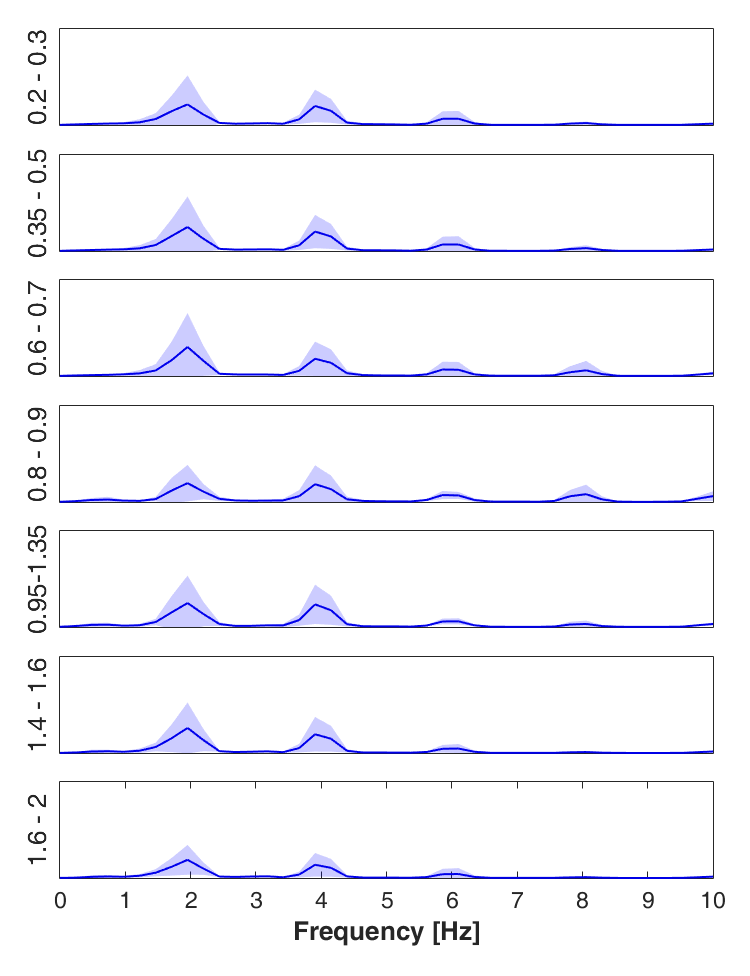
\includegraphics[width=1.\linewidth]{widmo_2Hz.png}
		\caption{Power spectrum for stimulation of 2 Hz.}
		\label{rys:widmo_2Hz}
	\end{subfigure}
	
\end{figure}
\begin{figure}[H]\ContinuedFloat		
	
	\begin{subfigure}{.5\textwidth}
		\centering
		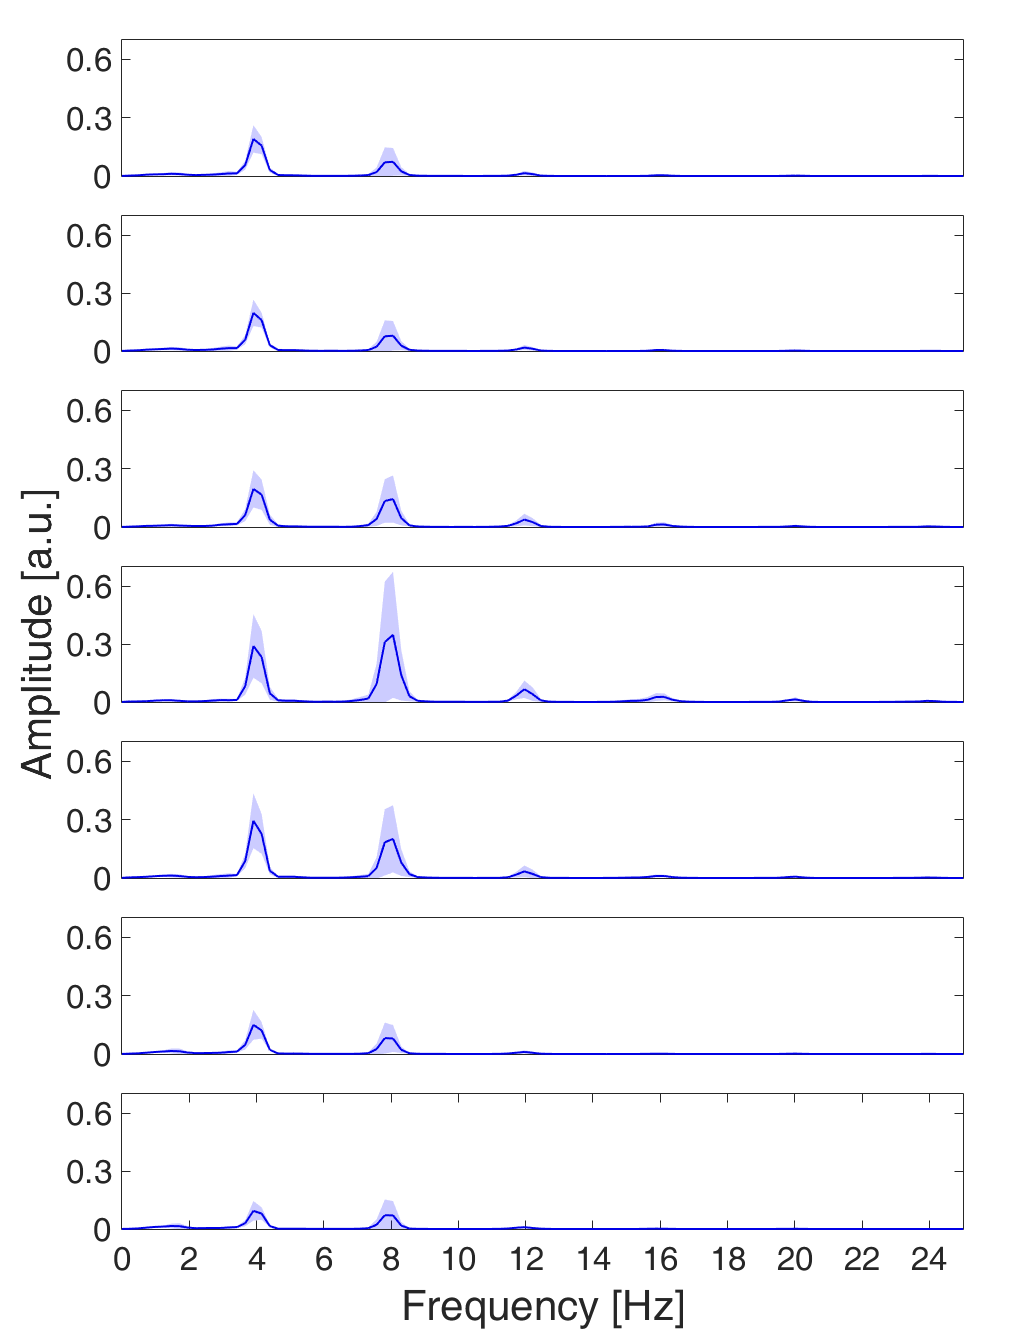
\includegraphics[width=1.\linewidth]{widmo_4Hz.png}
		\caption{Power spectrum for stimulation of 4 Hz.}
		\label{rys:widmo_4Hz}
	\end{subfigure}
	\begin{subfigure}{.5\textwidth}
		\centering
		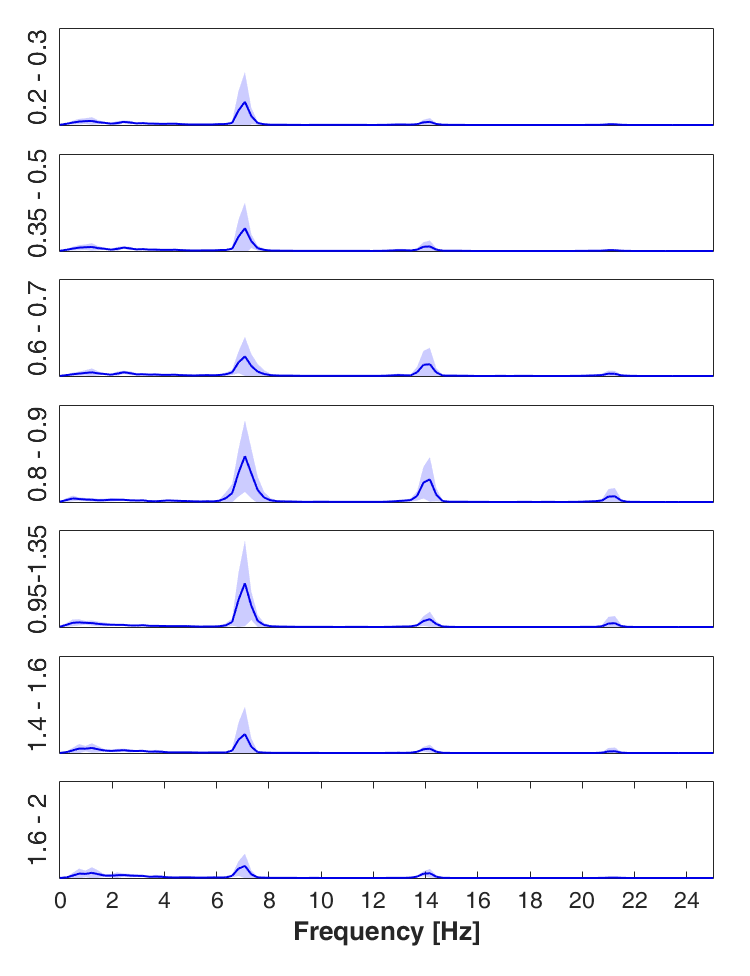
\includegraphics[width=1.\linewidth]{widmo_7Hz.png}
		\caption{Power spectrum for stimulation of 7 Hz.}
		\label{rys:widmo_7Hz}
	\end{subfigure}
		
		
	\begin{subfigure}{.5\textwidth}
		\centering
		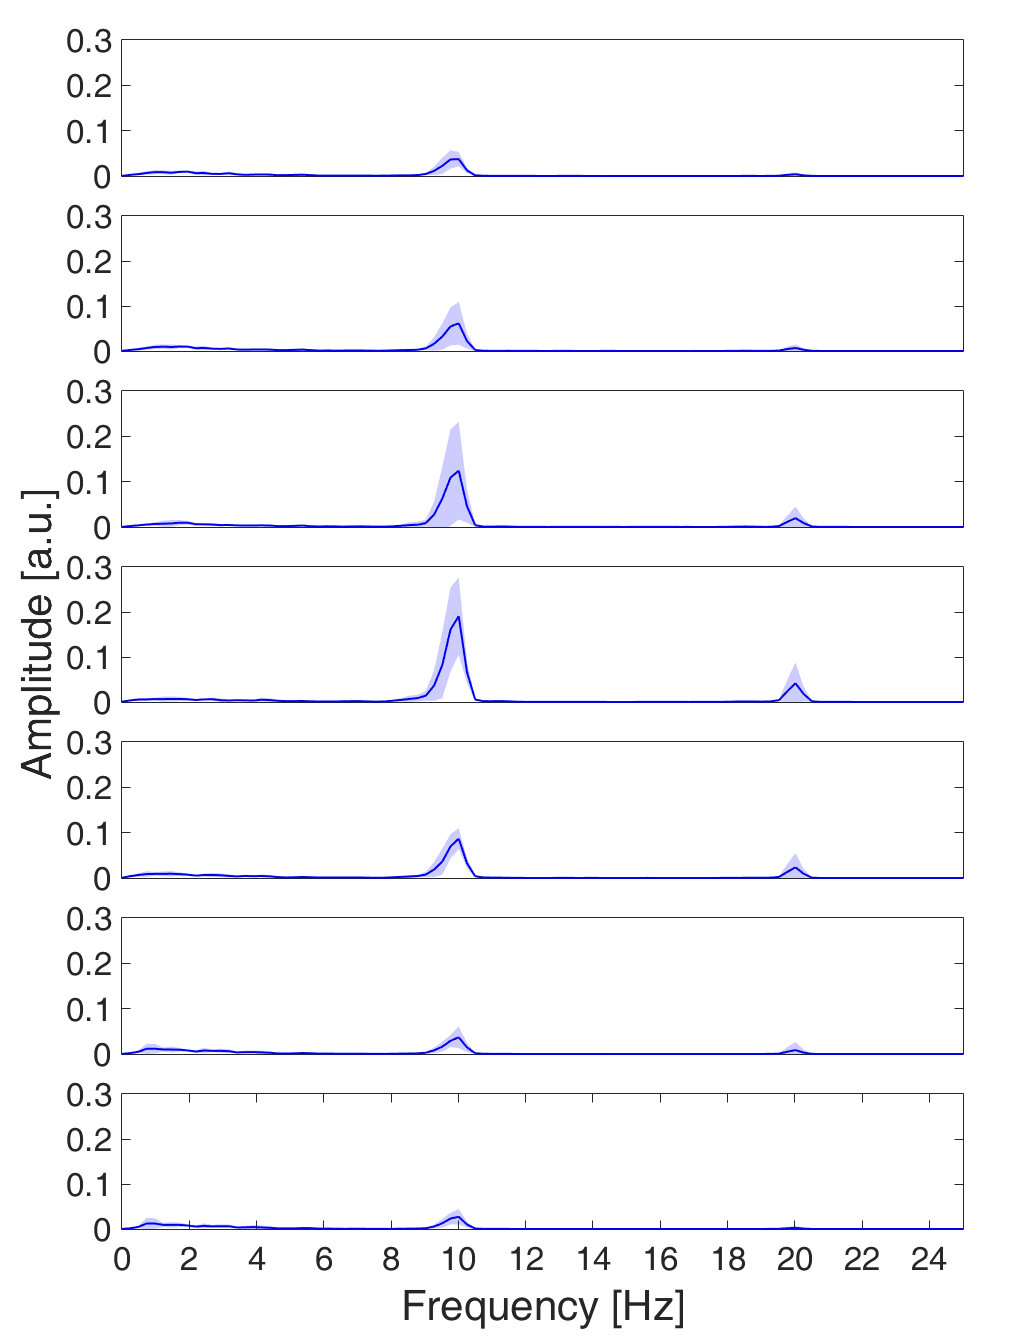
\includegraphics[width=1.\linewidth]{widmo_10Hz.png}
		\caption{Power spectrum for stimulation of 10 Hz.}
		\label{rys:widmo_10Hz}
	\end{subfigure}
	\begin{subfigure}{.5\textwidth}
		\centering
		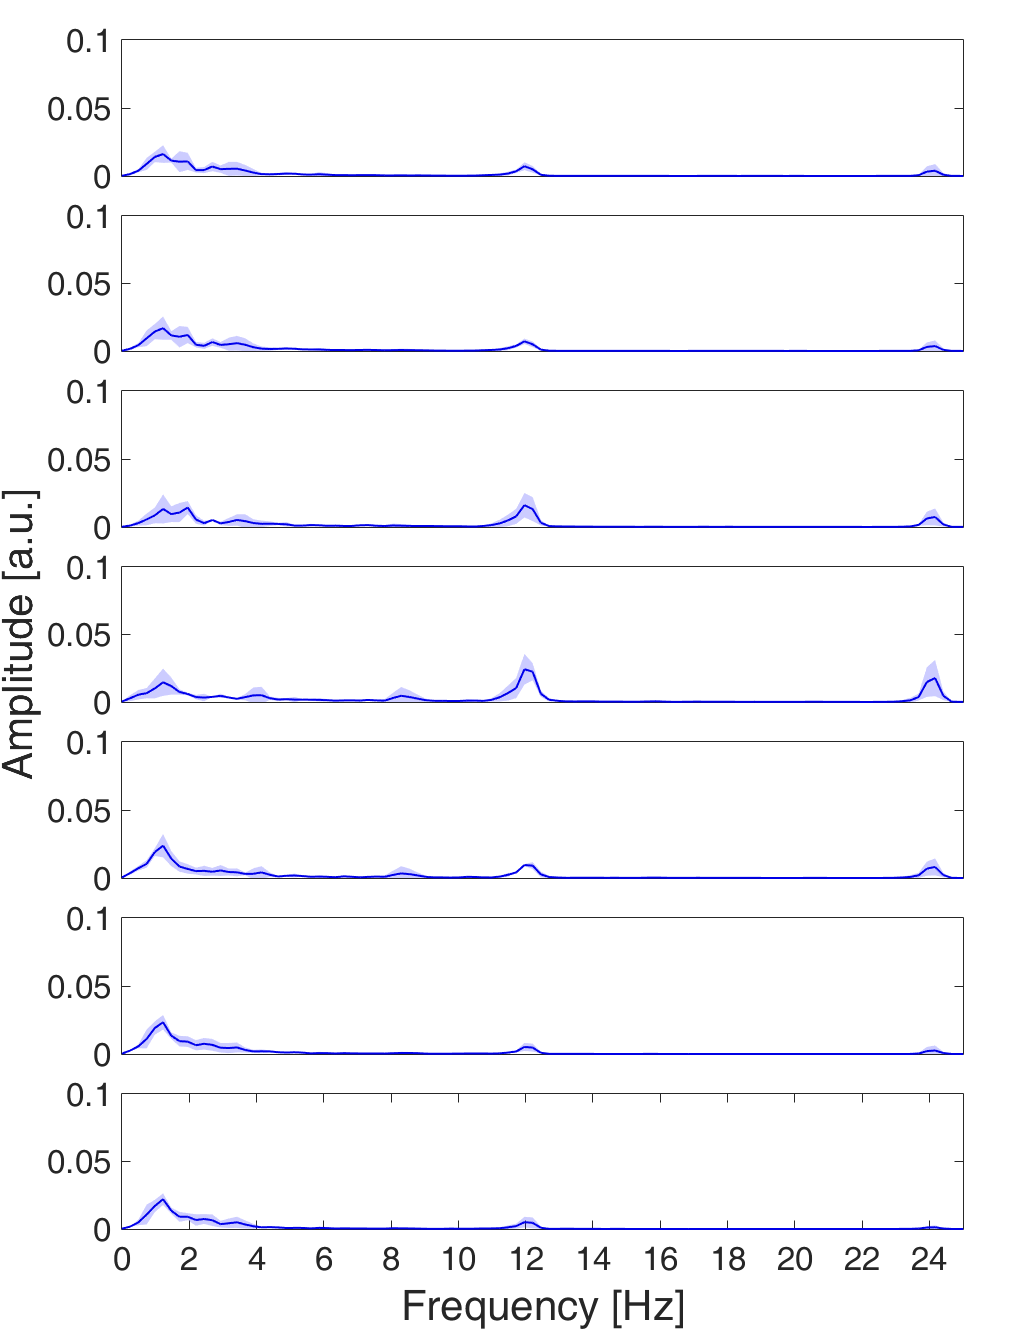
\includegraphics[width=1.\linewidth]{widmo_12Hz.png}
		\caption{Power spectrum for stimulation of 12 Hz.}
		\label{rys:widmo_12Hz}
	\end{subfigure}
	
	\caption{Power spectrum calculated for average by 40 trials for each animal. Blue intervals represent standard deviations by the animals. Y axis is different for all subfigures.}
	\label{rys:srednie_widmo}
	
\end{figure}    
\section{Analysis of current source density}
Current source density analysis is shown in Figure \ref{rys:csd}. For stimulation of 1 and 2 Hz there is a change in polarization to each repetition of stimulus. For stimulation of frequency higher than 2 Hz there is a change of polarization just after end of stimulation (around 5.1~s). 


	\begin{figure}[H]
	\begin{subfigure}{.5\textwidth}
		\centering
		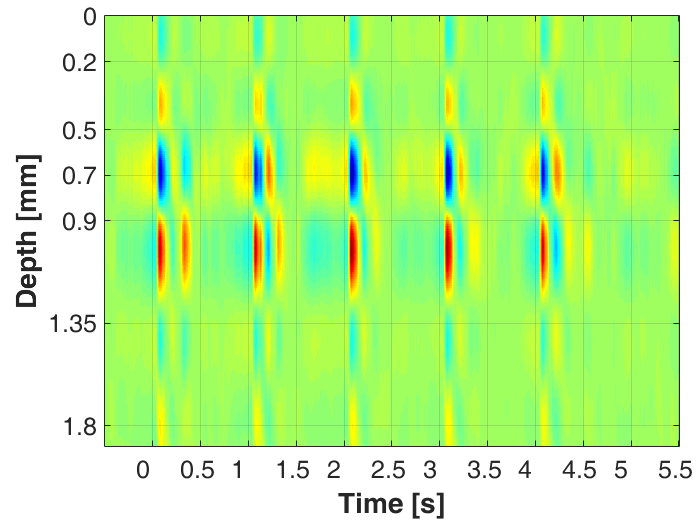
\includegraphics[width=1.\linewidth]{csd_1Hz_5s.png}
		\caption{CSD for stimulation of 1 Hz.}
		\label{rys:csd_1Hz}
	\end{subfigure}%
	\begin{subfigure}{.5\textwidth}
		\centering
		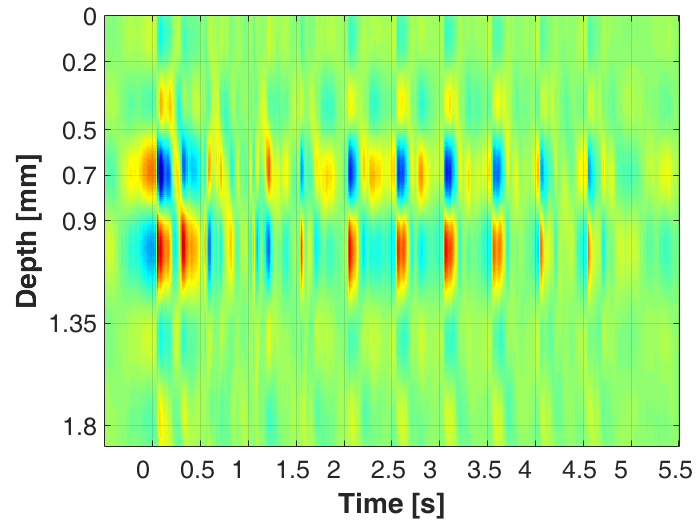
\includegraphics[width=1.\linewidth]{csd_2Hz_5s.png}
		\caption{CSD for stimulation of 2 Hz.}
		\label{rys:csd_2Hz}
	\end{subfigure}
	
	\begin{subfigure}{.5\textwidth}
		\centering
		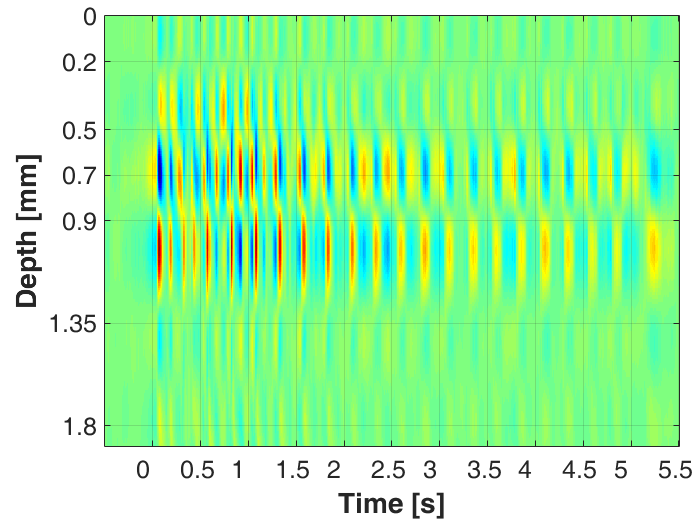
\includegraphics[width=1.\linewidth]{csd_4Hz_5s.png}
		\caption{CSD for stimulation of 4 Hz.}
		\label{rys:csd_4Hz}
	\end{subfigure}
	\begin{subfigure}{.5\textwidth}
		\centering
		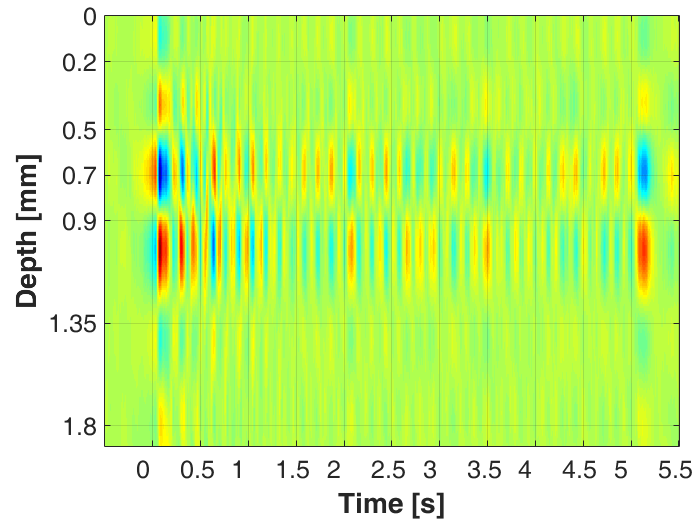
\includegraphics[width=1.\linewidth]{csd_7Hz_5s.png}
		\caption{CSD for stimulation of 7 Hz.}
		\label{rys:csd_7Hz}
	\end{subfigure}
	
\end{figure}
\begin{figure}[H]\ContinuedFloat
	
	\begin{subfigure}{.5\textwidth}
		\centering
		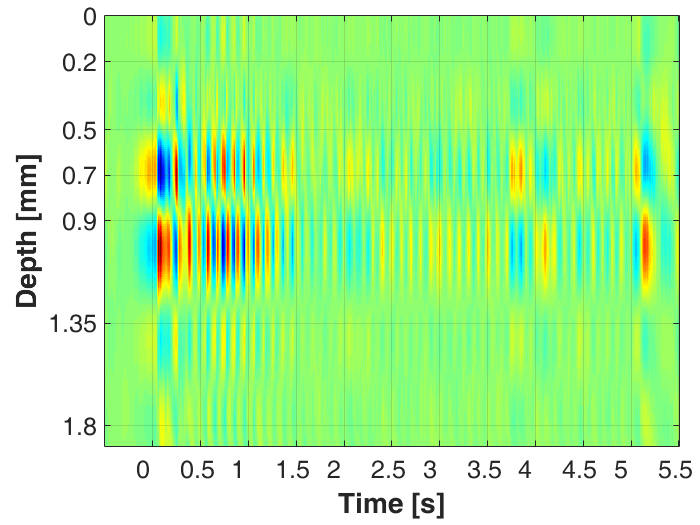
\includegraphics[width=1.\linewidth]{csd_10Hz_5s.png}
		\caption{CSD for stimulation of 10 Hz.}
		\label{rys:csd_10Hz}
	\end{subfigure}
	\begin{subfigure}{.5\textwidth}
		\centering
		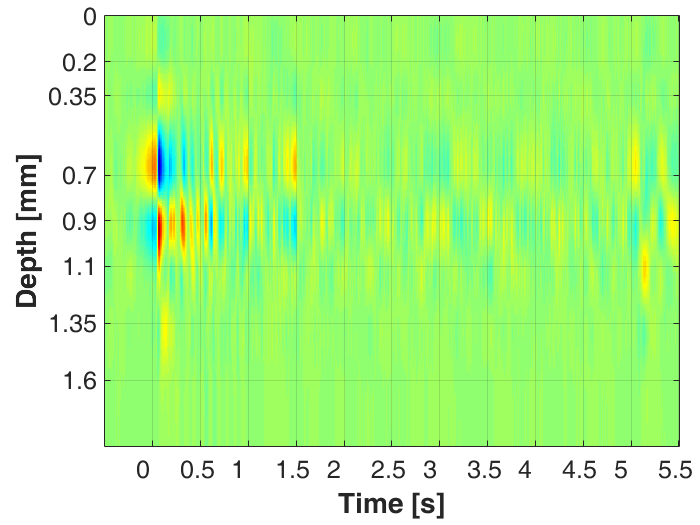
\includegraphics[width=1.\linewidth]{csd_12Hz_5s.png}
		\caption{CSD for stimulation of 12 Hz.}
		\label{rys:csd_12Hz}
	\end{subfigure}
	
	\caption{All experiments averaged by 40 trials and CSD is performed. Point 0 s shows beginning of 5 s constant stimulation. Scale is from blue (source) to red (sink). Y axis is the same for all subfigures.}
	\label{rys:csd}
	
	\end{figure}

    
    \section{Analysis of laminar profile for stimulation with 1 Hz frequency}
    Vertically the reverse of potential in layer IV of VCx can be observed (Fig. \ref{rys:srednie_1Hz_1s}). Granular layer (always 4. subfigure) is characterized by the most diverse response to the stimulation within this group of animals. It can be noticed that first peak of response is stable whereas second peak is more varied. 
	\begin{figure}[H]
	\begin{subfigure}{.5\textwidth}
		\centering
		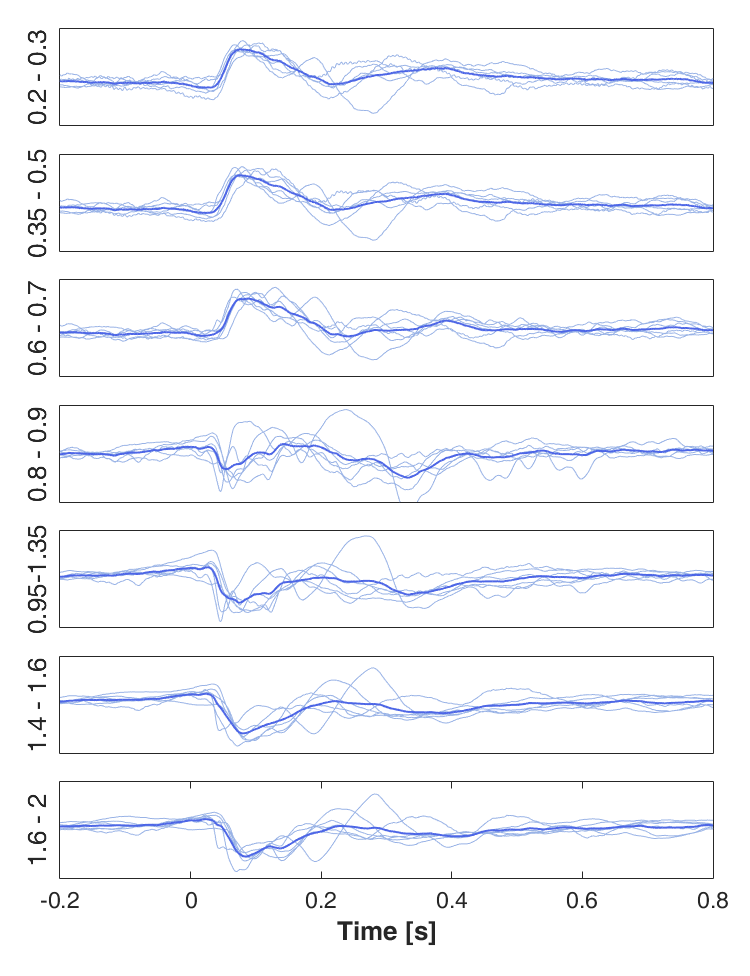
\includegraphics[width=1.\linewidth]{srednie_1Hz_linie.png}
		\caption{}
		\label{rys:srednie_1Hz_linie}
	\end{subfigure}%
	\begin{subfigure}{.5\textwidth}
		\centering
		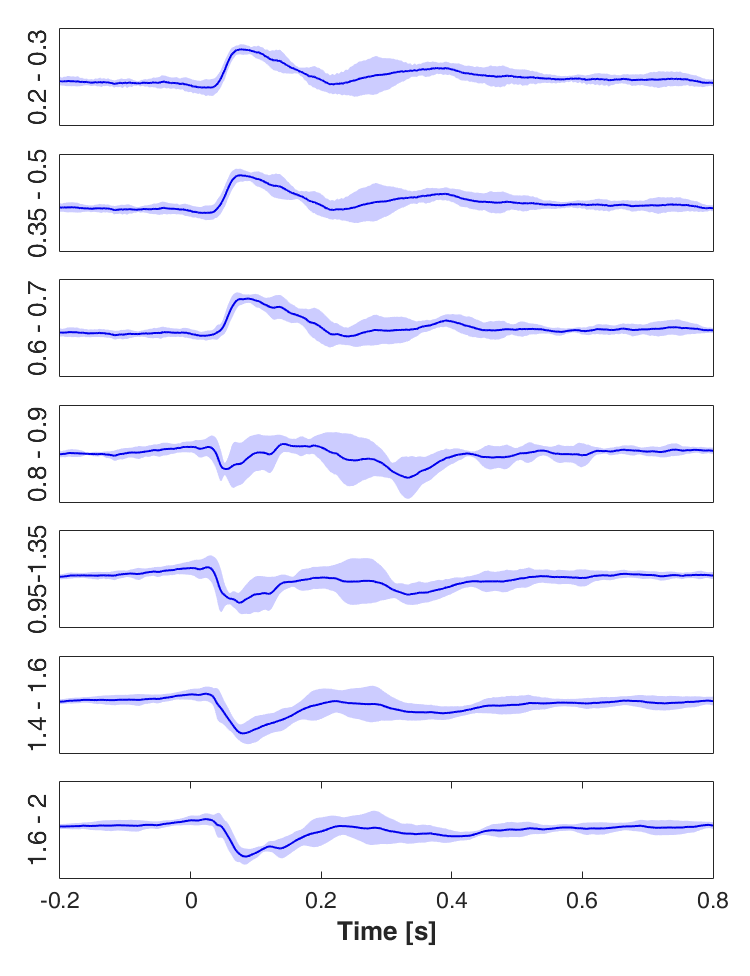
\includegraphics[width=1.\linewidth]{srednie_1Hz_std.png}
		\caption{}
		\label{rys:srednie_1Hz_std}
	\end{subfigure}

  \caption{Laminar profile in function of depth of the electrode for 1 Hz stimulation. All experiments averaged by 40 trials in time domain -- bold line. Single animals are presented in two ways: by separated lines (\ref{rys:srednie_1Hz_linie}) or by the standard deviation (\ref{rys:srednie_1Hz_std}). Point 0 s shows beginning of 5 s constant stimulation (here only 0.8 s is shown). Y axis is the same for both subfigures. }
  \label{rys:srednie_1Hz_1s}
\end{figure}

In the Figure \ref{rys:profil_1Hz_amp} laminar profile of amplitude in dependence of depth of the electrode is shown. Amplitude of the first peak is very similar among animals and there is clear change of sign between third and forth channel (Fig. \ref{rys:profil_1Hz_amp1}). Amplitude of the second peak is characterized by a high variance and there is not difference between layers (Fig. \ref{rys:profil_1Hz_amp2}).
  
\begin{figure}[H]
	\begin{subfigure}{.5\textwidth}
		\centering
		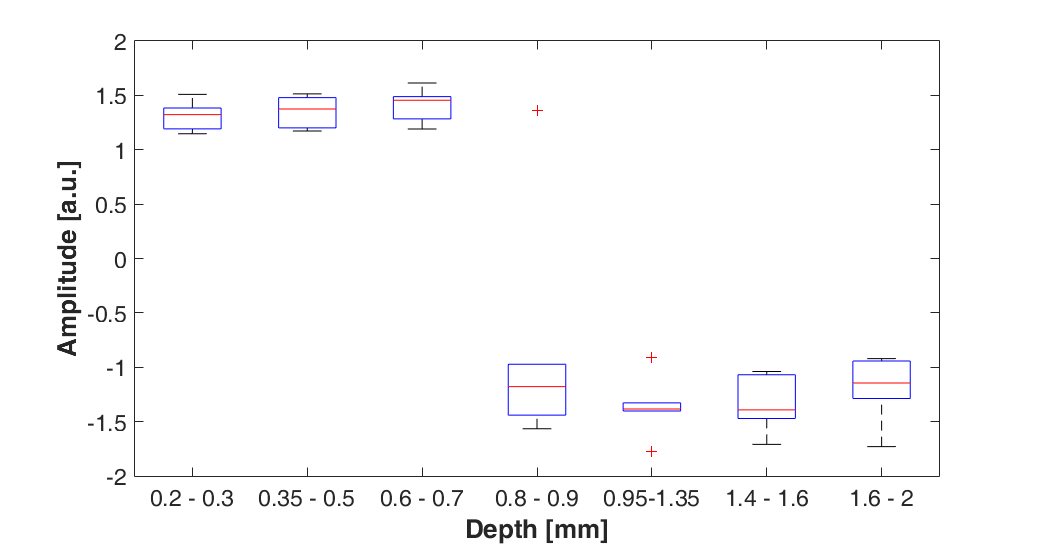
\includegraphics[width=1.\linewidth]{profile_1Hz_amp.png}
		\caption{Amplitude of the first peak.}
		\label{rys:profil_1Hz_amp1}
	\end{subfigure}%
	\begin{subfigure}{.5\textwidth}
		\centering
		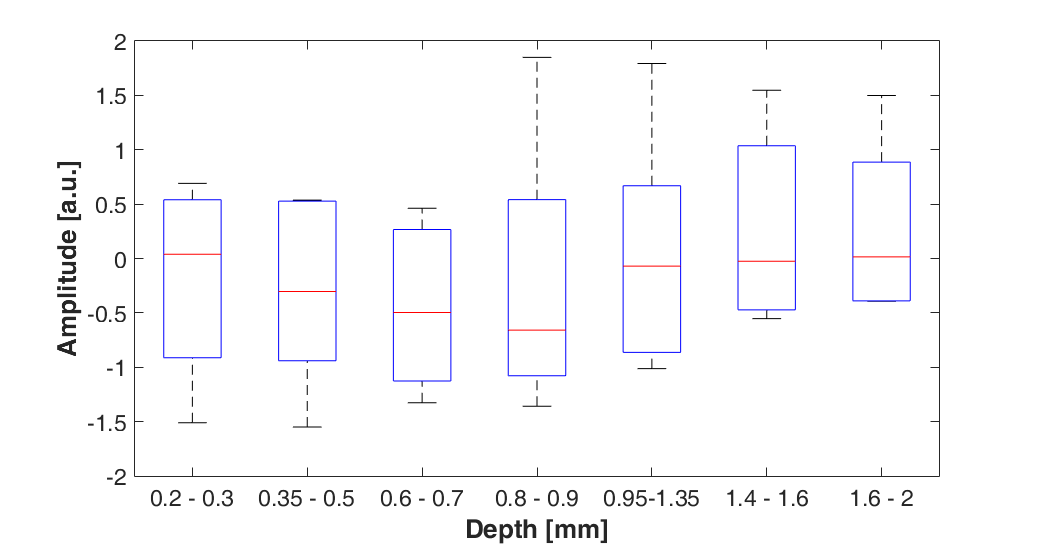
\includegraphics[width=1.\linewidth]{profile_1Hz_amp2.png}
		\caption{Amplitude of the second peak.}
		\label{rys:profil_1Hz_amp2}
	\end{subfigure}
	
	\caption{Amplitude of the averaged signal in function of the depth of the electrode for stimulation of 1 Hz. On the left there is an amplitude of first peak  (blue extremum in Fig. \ref{rys:piki_1Hz}), on the right -- amplitude of second peak (red extremum in Fig. \ref{rys:piki_1Hz}). Blue section is a 95\% confidence interval, red line is a mediana, red pluses are outliers.}
	\label{rys:profil_1Hz_amp}
\end{figure}

In the Figure \ref{rys:profil_1Hz_wid} laminar profile of amplitude of the peak fundamental and frequency and second harmonic in dependence of depth of the electrode is shown. Amplitude of the first peak is the biggest for fifth channel than for the others (Fig. \ref{rys:profil_1Hz_wid1}). Amplitude of the second peak is constant for all channels except the forth one. This channel also has the highest variance (Fig. \ref{rys:profil_1Hz_wid2}).


\begin{figure}[H]
	\begin{subfigure}{.5\textwidth}
		\centering
		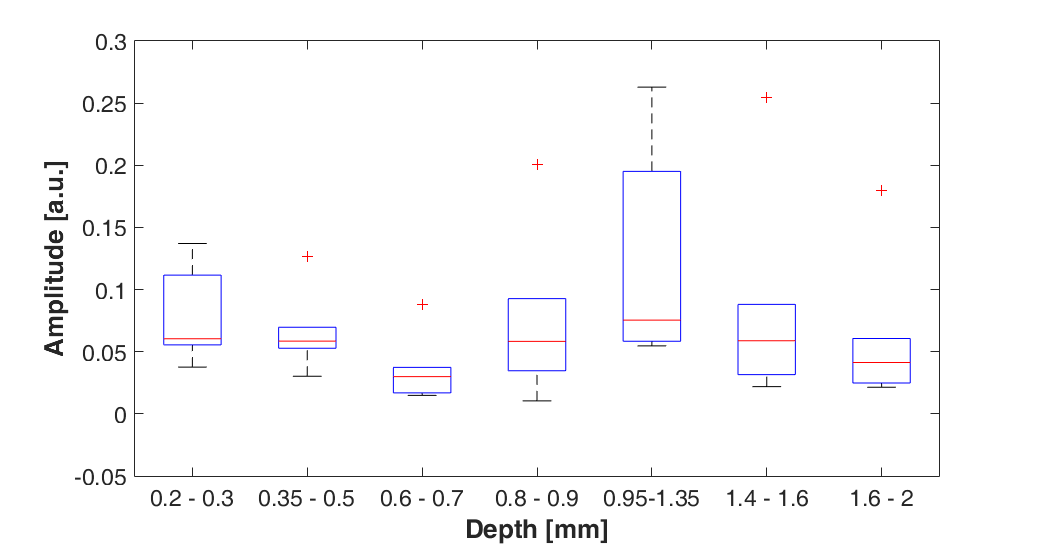
\includegraphics[width=1.\linewidth]{profile_1Hz_wid.png}
		\caption{An amplitude of peak in fundamental frequency.}
		\label{rys:profil_1Hz_wid1}
	\end{subfigure}%
	\begin{subfigure}{.5\textwidth}
		\centering
		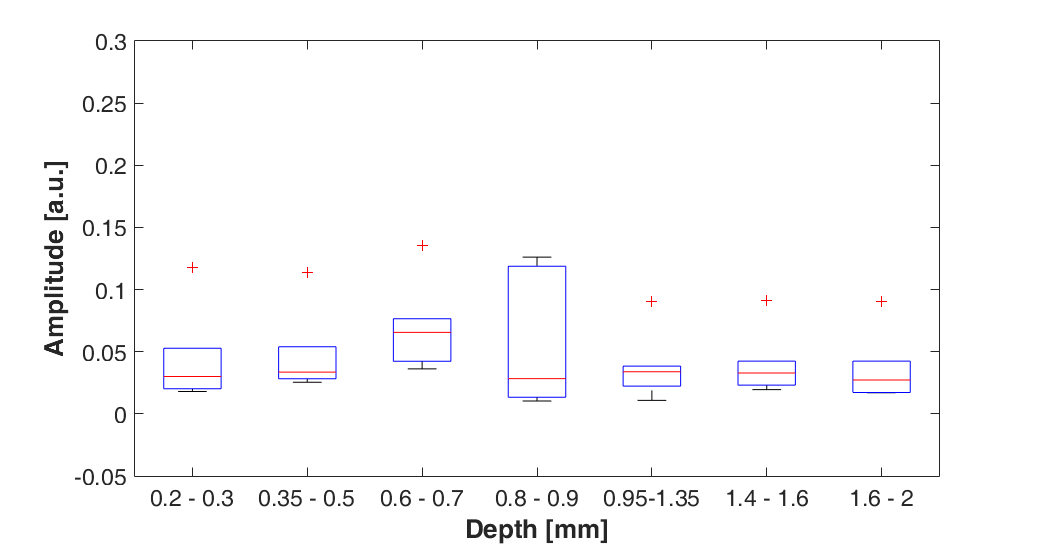
\includegraphics[width=1.\linewidth]{profile_1Hz_wid2.png}
		\caption{An amplitude of peak in the second harmonic.}
		\label{rys:profil_1Hz_wid2}
	\end{subfigure}
	
	\caption{Laminar profile of frequency domain in function of depth of the electrode for 1 Hz stimulation. On the left there is an amplitude of peak in fundamental frequency, on the right -- amplitude of second harmonic. Blue section is a 95\% confidence interval, red line is a mediana, red pluses are outliers. }
	\label{rys:profil_1Hz_wid}
\end{figure}


 
 \section{Laminar analysis for stimulation with 2 Hz frequency}
  
    In the Figure \ref{rys:profil_2Hz_amp} laminar profile of amplitude of response to stimulus in dependence of depth of the electrode for stimulation of 2 Hz is shown. Amplitude of the first peak is very similar among animals except channel 4 where variance is the biggest. (Fig. \ref{rys:profil_2Hz_amp1}). Tendency of amplitude of the second peak is like for 1 Hz: it has a high variance and there is not difference between layers (Fig. \ref{rys:profil_2Hz_amp2}).
  
 	\begin{figure}[H]
 	\begin{subfigure}{.5\textwidth}
 		\centering
 		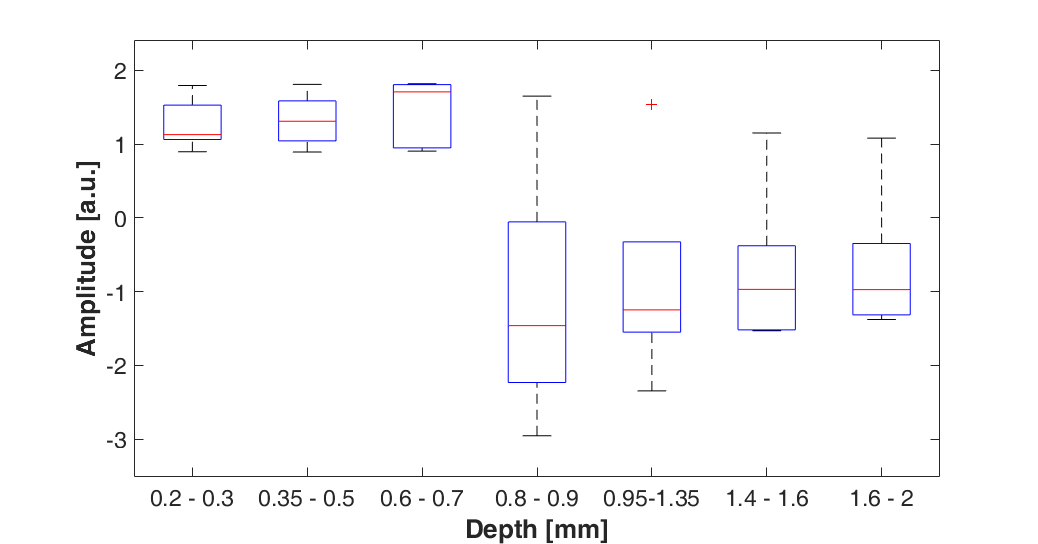
\includegraphics[width=1.\linewidth]{profile_2Hz_amp.png}
 		\caption{}
 		\label{rys:profil_2Hz_amp1}
 	\end{subfigure}%
 	\begin{subfigure}{.5\textwidth}
 		\centering
 		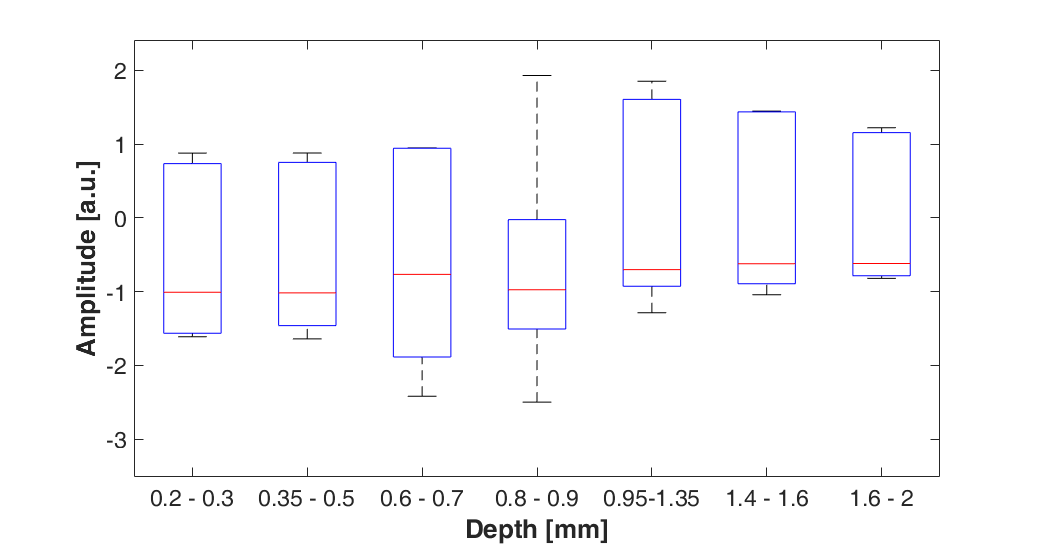
\includegraphics[width=1.\linewidth]{profile_2Hz_amp2.png}
 		\caption{}
 		\label{rys:profil_2Hz_amp2}
 	\end{subfigure}
 	
 	\caption{Laminar profile in function of depth of the electrode for 2 Hz stimulation.}
 	\label{rys:profil_2Hz_amp}
 \end{figure}

 In the Figure \ref{rys:profil_2Hz_wid} laminar profile of amplitude of peak in 2 and 4 Hz in dependence of depth of the electrode for stimulation of 2 Hz is shown. There is no clear difference for amplitude of the first peak. (Fig. \ref{rys:profil_2Hz_wid1}). Median for second peak is the lowest for forth channel but all channels have the same, high variance (Fig. \ref{rys:profil_2Hz_wid2}).
 
   	\begin{figure}[H]
  	\begin{subfigure}{.5\textwidth}
  		\centering
  		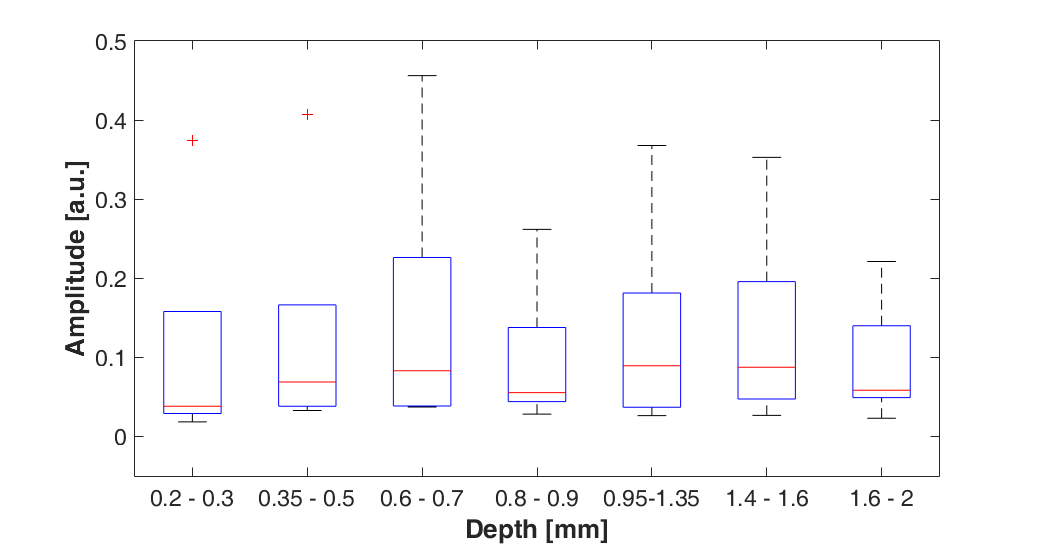
\includegraphics[width=1.\linewidth]{profile_2Hz_wid.png}
  		\caption{}
  		\label{rys:profil_2Hz_wid1}
  	\end{subfigure}%
  	\begin{subfigure}{.5\textwidth}
  		\centering
  		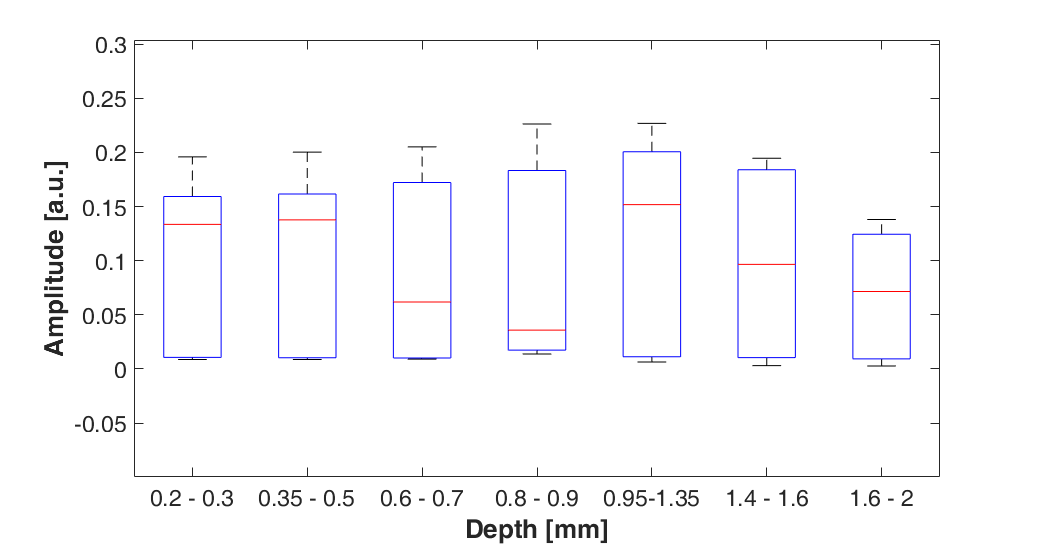
\includegraphics[width=1.\linewidth]{profile_2Hz_wid2.png}
  		\caption{}
  		\label{rys:profil_2Hz_wid2}
  	\end{subfigure}
  	
  	\caption{Laminar profile in function of depth of the electrode for 2 Hz stimulation.}
  	\label{rys:profil_2Hz_wid}
  \end{figure}
  
\section{Laminar analysis for stimulation with 4 Hz frequency} 
   	\begin{figure}[H]
	\begin{subfigure}{.5\textwidth}
		\centering
		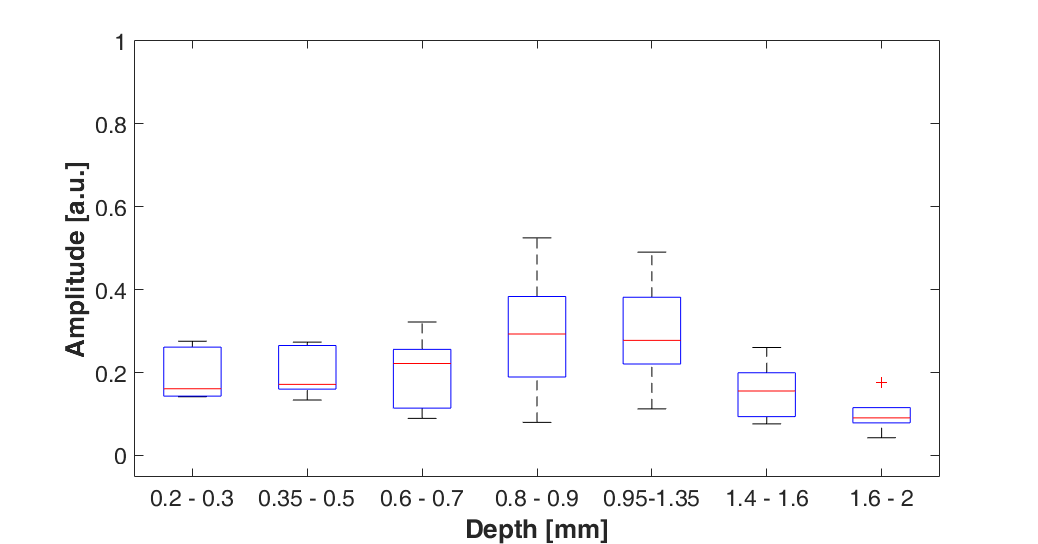
\includegraphics[width=1.\linewidth]{profile_4Hz_wid.png}
		\caption{}
		\label{rys:profil_4Hz_wid1}
	\end{subfigure}%
	\begin{subfigure}{.5\textwidth}
		\centering
		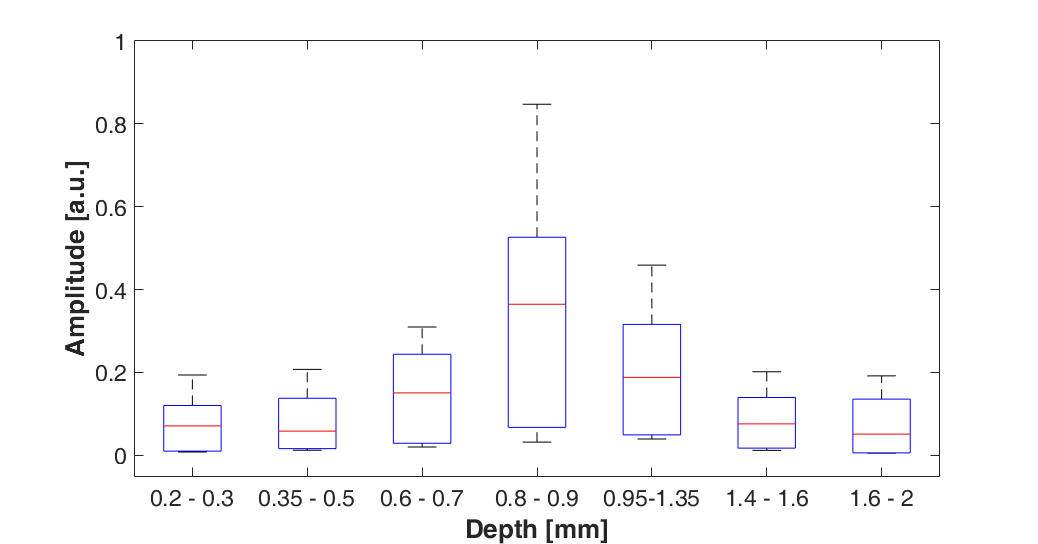
\includegraphics[width=1.\linewidth]{profile_4Hz_wid2.png}
		\caption{}
		\label{rys:profil_4Hz_wid2}
	\end{subfigure}
	
	\caption{Laminar profile in function of depth of the electrode for 4 Hz stimulation.}
	\label{rys:profil_4Hz_wid}
\end{figure}
\section{Laminar analysis for stimulation with 7 Hz frequency}  
   	\begin{figure}[H]
	\begin{subfigure}{.5\textwidth}
		\centering
		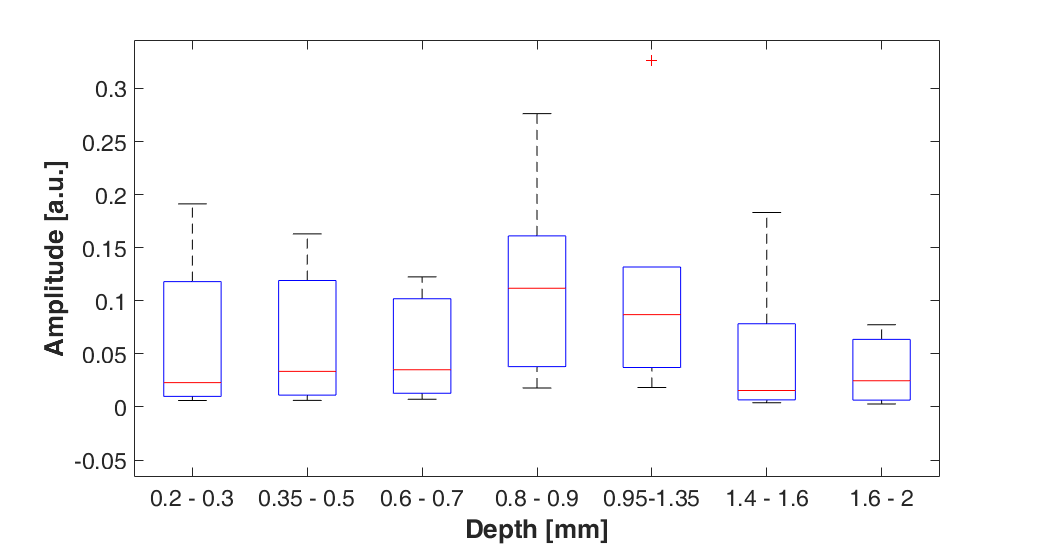
\includegraphics[width=1.\linewidth]{profile_7Hz_wid.png}
		\caption{}
		\label{rys:profil_7Hz_wid1}
	\end{subfigure}%
	\begin{subfigure}{.5\textwidth}
		\centering
		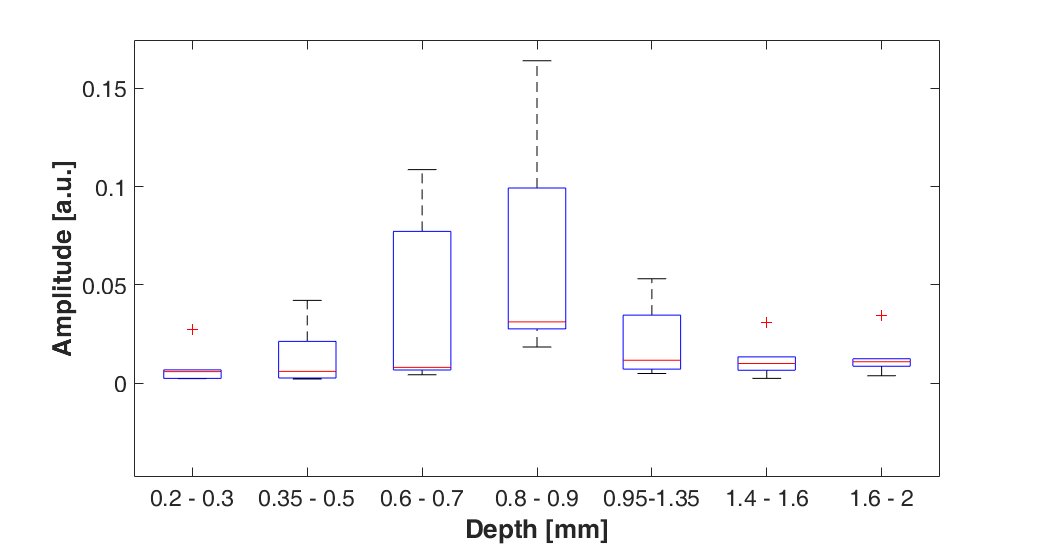
\includegraphics[width=1.\linewidth]{profile_7Hz_wid2.png}
		\caption{}
		\label{rys:profil_7Hz_wid2}
	\end{subfigure}
	
	\caption{Laminar profile in function of depth of the electrode for 7 Hz stimulation.}
	\label{rys:profil_7Hz_wid}
\end{figure}
\section{Laminar analysis for stimulation with 10 Hz frequency}  
   	\begin{figure}[H]
	\begin{subfigure}{.5\textwidth}
		\centering
		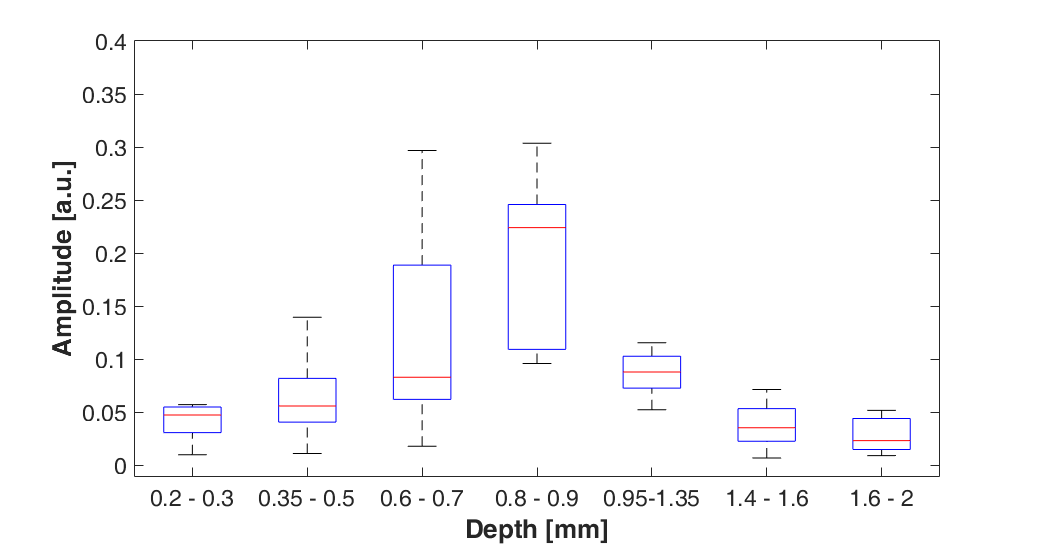
\includegraphics[width=1.\linewidth]{profile_10Hz_wid.png}
		\caption{}
		\label{rys:profil_10Hz_wid1}
	\end{subfigure}%
	\begin{subfigure}{.5\textwidth}
		\centering
		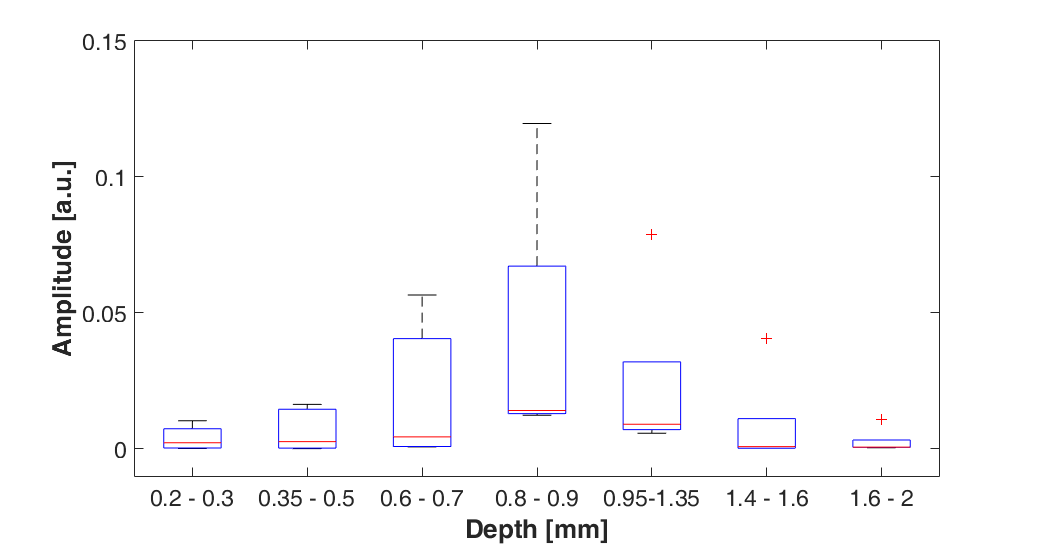
\includegraphics[width=1.\linewidth]{profile_10Hz_wid2.png}
		\caption{}
		\label{rys:profil_10Hz_wid2}
	\end{subfigure}
	
	\caption{Laminar profile in function of depth of the electrode for 10 Hz stimulation.}
	\label{rys:profil_10Hz_wid}
\end{figure}
\section{Laminar analysis for stimulation with 12 Hz frequency}  
   	\begin{figure}[H]
	\begin{subfigure}{.5\textwidth}
		\centering
		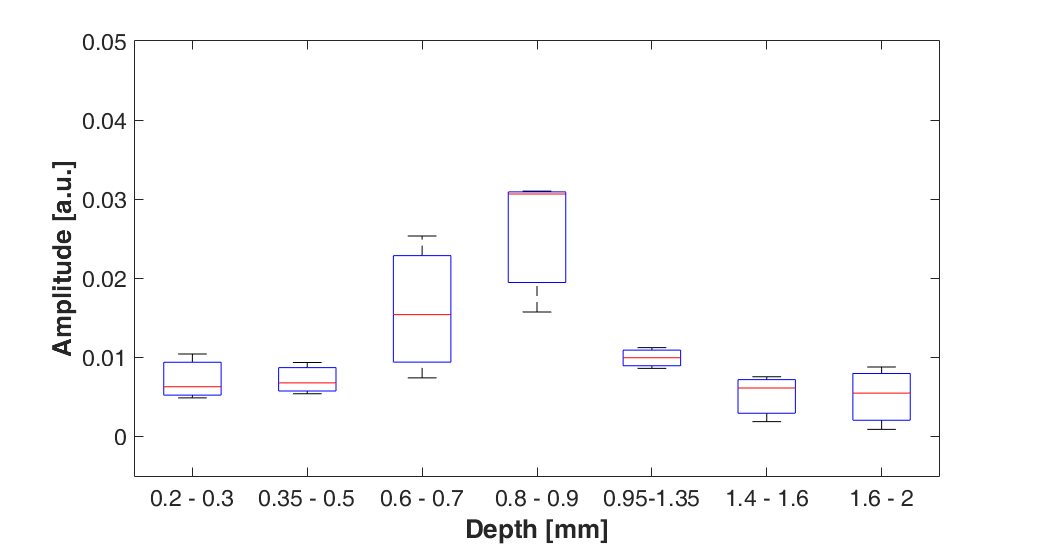
\includegraphics[width=1.\linewidth]{profile_12Hz_wid.png}
		\caption{}
		\label{rys:profil_12Hz_wid1}
	\end{subfigure}%
	\begin{subfigure}{.5\textwidth}
		\centering
		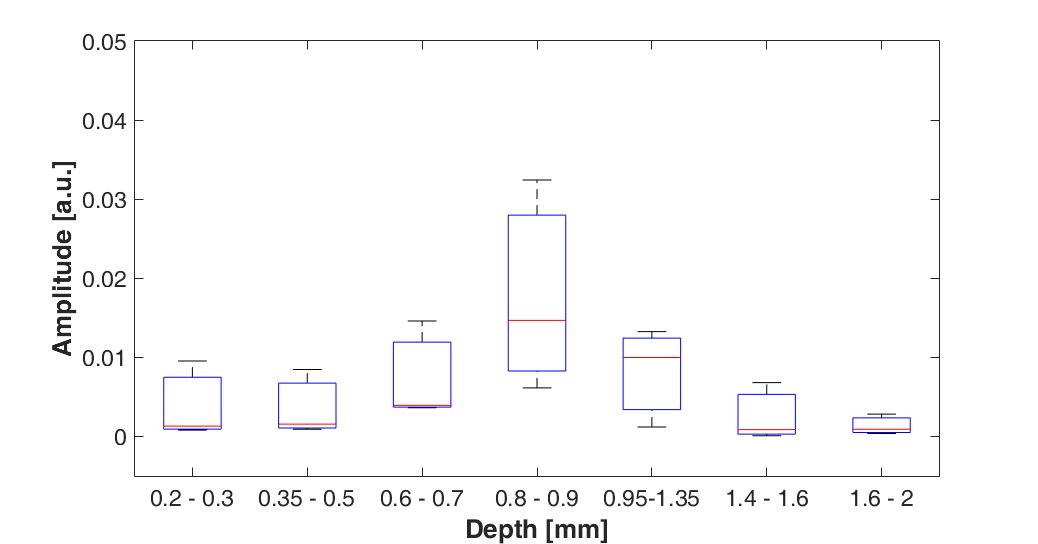
\includegraphics[width=1.\linewidth]{profile_12Hz_wid2.png}
		\caption{}
		\label{rys:profil_12Hz_wid2}
	\end{subfigure}
	
	\caption{Laminar profile in function of depth of the electrode for 12 Hz stimulation.}
	\label{rys:profil_12Hz_wid}
\end{figure}
    \chapter{Discussion}
    
    First of all, it is worth mentioning that even though all recordings were performed on the same structure, using the same electrode, brain anatomy differs between subjects. Individual channels were chosen for analysis based on the pattern of visual potential so there is no guarantee that one channel represents exactly the same structure for every animal. The same concerns the method of recording signal---local field potential is spatially an inaccurate method because it gathers signal from quite a big area of the brain, possibly spanning over multiple structures. On the other hand, this experiment was performed on a group of six animals and the obtained results are coherent and repeatable. Especially the latter confirms that the conclusions are correct. 
    
    Analysis of averaged signal for 1 Hz and 2 Hz indicates that there is a clear difference in amplitude of the first peak between supra- and infragranular layers. It can be a result of the fact that magnocellular channel enters from LGN mainly to layer IV of VCx and information from there propagates the further the bigger amplitude gets. For both stimulations there was a high variance of the amplitude of the second peak between animals, but there was no significant difference across the layers. Although the results of averaged potentials are similar for both low-frequency stimulations, there are substantial differences in the peaks for fundamental frequency and second harmonic. For 1 Hz stimulation channel 5 exhibited the highest amplitude and variance of fundamental frequency, while for 2 Hz stimulation channel 4 had the lowest value and variance. The same concerns second harmonic: for 1 Hz stimulation all channels had similar values except channel 4 which stood out having the highest variance. For 2 Hz stimulation the situation was quite opposite---channel 4 exhibited the lowest variance. Those contradictory effects may be a result of improper method of analysis. On the other hand, they could be due to high amplitude of low frequencies which are present in a sleeping animal so that low frequency of stimulation may be not enough to stand out (\cite{ja}).
    
    For stimulation with frequency higher than 2 Hz the amplitude of peak in averaged signal was not calculated because stimulus occurred to often to generate full response and it was not possible to determine the peak. During analysis in the frequency domain the same tendency for all frequencies was observed. It is noticeable already for fundamental frequency, but for second harmonic it is much more apparent: channel 4 is characterized by the biggest amplitude and has lower variance than other channels. It also may be a cause of magnocellular entrance in layer IV in VCx.
    
    

\printbibliography[heading=bibintoc]

\end{document}
